%\chapter{移动环境下支持QoS关联的组合服务Skyline计算}
\chapter{支持动态QoS关联的组合服务Skyline计算}

\section{引言}

近年来,随着移动网络的迅猛发展,以及越来越多移动设备和自主无人装置的出现,运行在这些设备或装置上的移动~Web~服务的数量也逐渐增加。这些设备通常具有移动的特性,比如持有手机的人会发生位置的变化,再比如执行任务的无人勘测车也会不断的移动去采集数据。由于这些设备的移动性,使得以这些设备为运行依托的Web服务也会具有移动的特性。这种移动的特征会导致服务之间的~QoS~ 关联值会随着提供Web 服务的设备的移动而发生变化,而已有的工作都没有考虑到这一点。

当服务之间的~QoS~关联值发生变化的时候,我们需要重新计算组合服务~Skyline,与此次同时,与每个抽象服务对应的~SAP~也要重新计算。然而,有些情况下,比如某些被标记为不可用的~QoS~关联(详见:\ref{S:SEC_CSKYCOMPUTING}节)的关联值变动范围很小的时候,它仍然会被其他服务或者是关联所支配,我们不需要去重新计算~SAP~以及组合服务~Skyline。 从而减少在组合服务代理上无意义的计算,提高组合服务代理的运行效率。

为了解决这个问题,我们希望为每一个~QoS~关联确定一个安全值范围(\underline{S}afe \underline{V}alue \underline{R}ange,~SVR),当一个关联值在这个范围内变动的时候,它的状态不变,换句话说,如果关联值变动之前,它是被标记为不可用状态(即关联被移除),那么变动之后,它依然是不可用状态,如果关联值变动之前,它是处于可用状态(即关联没有被移除),那么在变动之后,它依然处于可用状态,同时不使得其他处于可用状态的关联变为不可用。

当服务关联值的变化超出安全值范围的时候,我们需要重新计算~SAP~以及~CSKY~,当服务关联值的变化在安全值范围内的时候,我们需要分情况讨论:如果关联被标记为可用状态,无需重新计算~SAP~,但是无法确定是否需要重新计算~CSKY~,而如果关联被标记为不可用状态,那么无需重新计算~SAP~,也无需重新计算~CSKY~。

本章所关注的重点在于,如何为Web服务中的每一个关联确定安全值范围。

\section{背景}

\subsection{研究动机}

我们假设有一个地方发生了地震,如图~\ref{F:Fig_MobileScene}~所示的灾区。相关部门需要根据灾情分析报告来做出应急措施。为了达到这个目的,我们需要用到数据采集服务以及数据分析服务来帮助生成灾情分析报告。组合服务代理会根据该需求,生成包含数据采集服务以及数据分析服务的抽象组合服务,并为之选择出组合服务~Skyline:$\{\{A,D\},\{B,C\}\}$。服务~$A$~ 是由图中的勘测车提供的,服务~$B$~ 是由当地地震局提供的,服务~$C$~将数据采集服务传来的数据,稍作处理(对齐等操作)就打印出报告,而服务~$D$~还会根据数据采集服务传来的数据做一些分析,给出简单的建议,因此服务~$D$~ 的响应时间与数据的好坏有着很大的关系。通常,在灾区外围采集的数据并不是特别完整,越靠近灾区越好。因而当勘测车开入灾区后,得到相对完整的数据,使得服务~$D$~的处理时间降低,服务~$A$~与服务~$D$~存在~QoS~ 关联。我们假设只要勘测车在灾区中,提供的数据质量总是比在外边好的,因此只要勘测车在灾区中,~$D$~ 的关联~QoS~值总是比原来的低,除此之外,灾区中有些区域的网络还可以,有些区域网络很差,导致传输车的信号不稳定,而传输车为了保证自身的响应时间,他会将数据做一些处理,比如丢弃一些数据,但是丢弃后的数据仍比灾区外采集的要好,从而~$D$~的关联~QoS~值会发生波动。

\begin{figure}[!thb]
    \centering
    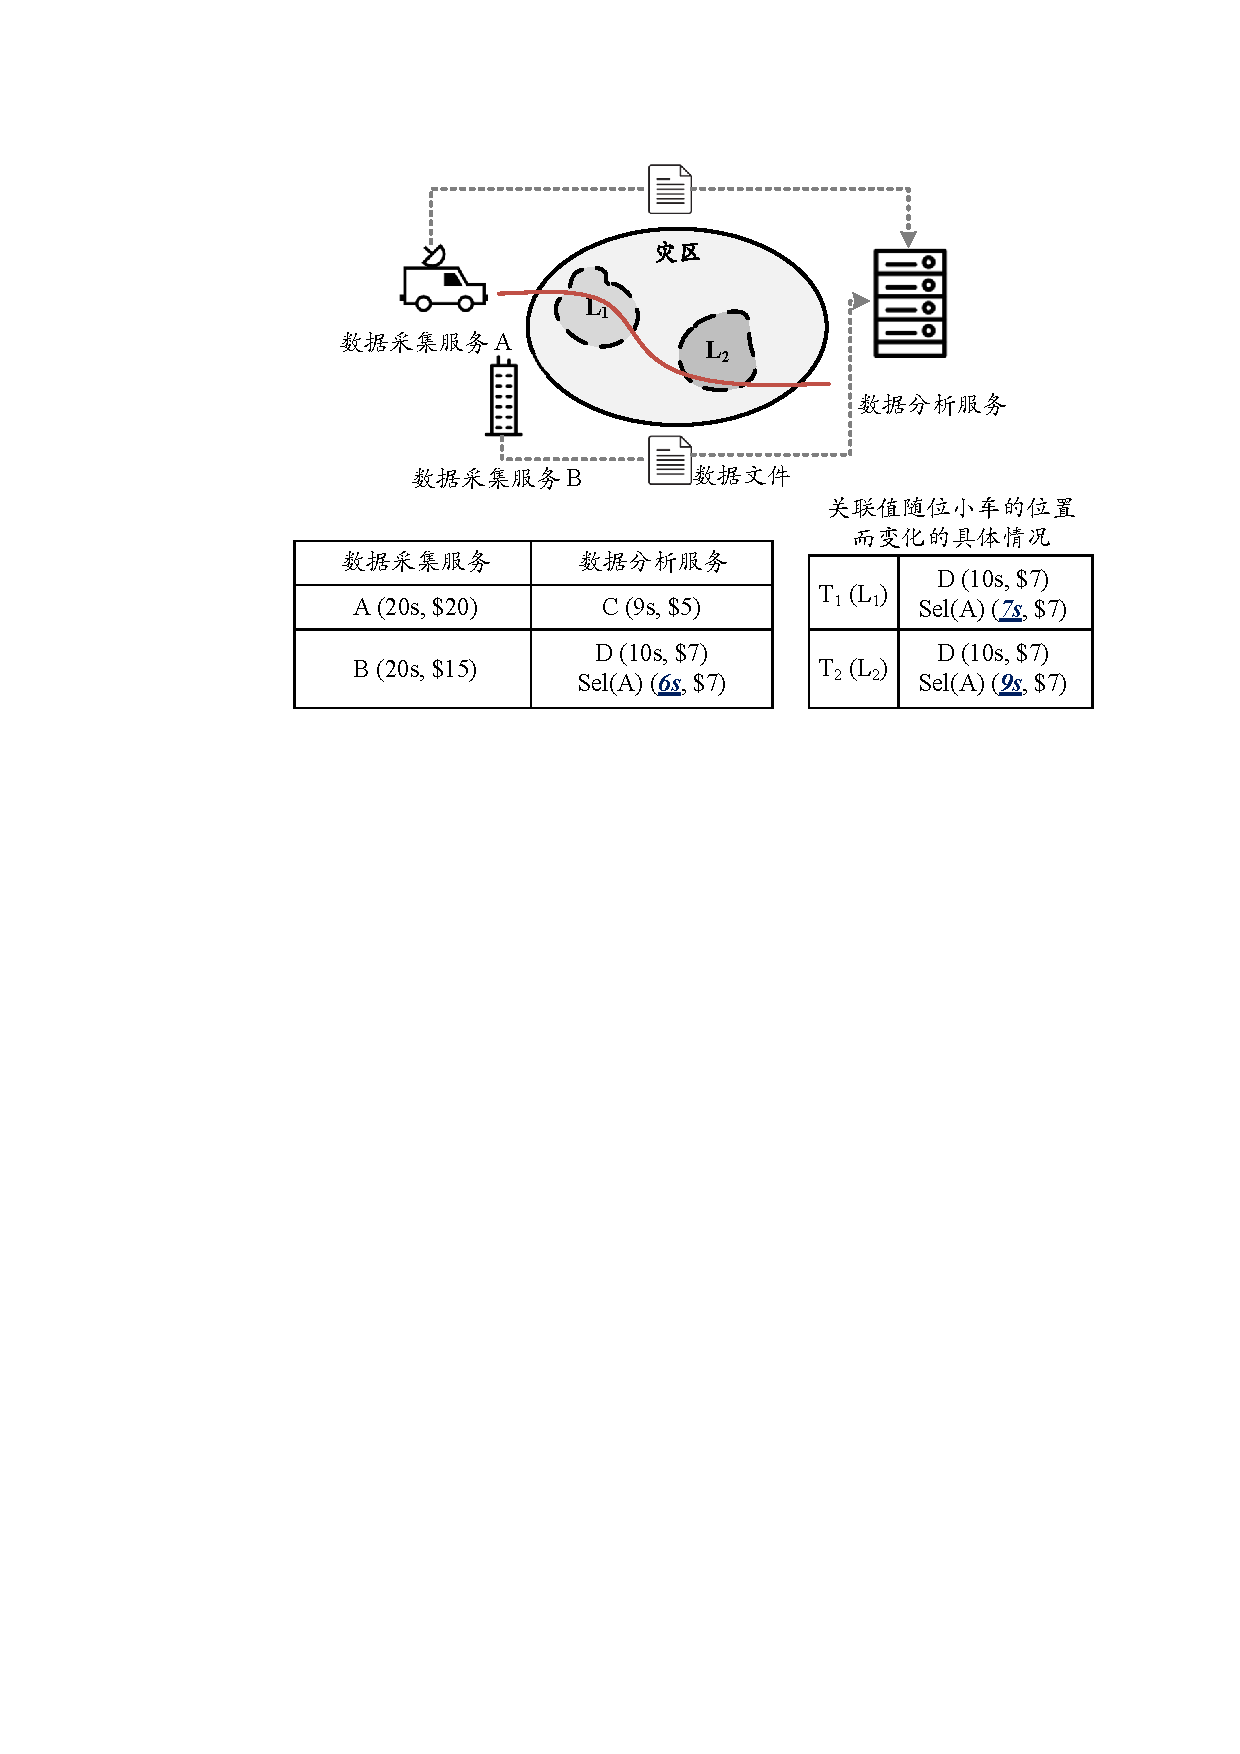
\includegraphics[width=0.9\textwidth]{./FIGs/Fig_MobileScene.pdf}
    \caption{移动Web服务}
    \label{F:Fig_MobileScene}
\end{figure}

在图~\ref{F:Fig_MobileScene}~中,勘测车按照红色线标识的路线行驶并采集数据,在~T$_{1}$~时刻,勘测车处于~L$_{1}$~ 位置,~$A$~ 与~$D$~ 的关联值变为$7s$,在~T$_{2}$~时刻,勘测车处于~L$_{2}$~ 位置,~$A$~ 与~$D$~的关联值变为$9s$。 我们发现在~T$_{1}$~时刻,不需要重新计算~SAP~ 和~CSKY~,只有到~T$_{2}$~的时候才需要重新计算。

\subsection{预备知识}


有关服务~QoS~关联,服务,服务组合的模型在~\ref{S:SEC_CorrModel}~节中已经给出了详细的定义,这里不再赘述。但为了方便描述本章的问题,我们还需要补充一些新的定义。

\begin{definition}[安全值范围,SVR]

一个~\emph{QoS}~关联$c$的安全值范围~\emph{SVR}$(c)=[lb,\ ub]$,lb~是关联值的下界(\emph{Low Bound}),ub~是关联值的上界(\emph{Upper Bound}),且关联值在这个范围内变动的时候,~\emph{QoS}~ 关联的状态保持不变,同时不影响其他关联的状态。

\end{definition}

\begin{definition}[在非关联属性上的支配]

假设~\emph{QoS}~有~$d$~维属性,其中~QoS~关联发生在第~$i$~维上,那么非关联的~\emph{QoS}~属性为$\{q_{1}$,$\cdots$, $q_{i-1}$, $q_{i+1}$,$\cdots$, $q_{d}$$\}$,记为~\emph{QoS$_{\overline{i}}$}。如果在~ \emph{QoS$_{\overline{i}}$}~ 上,$x$~支配~$y$,我们就称$x$~ 在非关联属性上支配~$y$,记为~$x \succ_{\overline{i}} y$。

\end{definition}

表~\ref{T:Tab_Notations2}~中定义了本章接下来的部分用到的一些符号。

%表格:服务集合
\begin{table}[!thb]
\centering  % 表居中
\begin{tabular}{|c|m{3in}<\centering|}  % {} 表示各列元素对齐方式,left-l,right-r,center-c
\hline
\textbf{\emph{符号}} & \textbf{\emph{解释}}
\\ \hline\hline
isRem($c$) & 判断$c$是否被标记为删除(也即不可用状态)。
\\ \hline
remType($c$) & 返回$c$是依据哪些剪枝规则删除的。 如果是依据定理~\ref{TH:Theo_Rule2}~ 以及引理~\ref{LM:Lemma_Rule3}~删除的,结果返回0,如果是依据定理~\ref{TH:Theo_Rule4}~ 以及引理~\ref{LM:Lemma_Rule5}~ 删除的,返回1。
\\ \hline
getAftedS($c$) & 返回关联$c$所指向的服务。
\\ \hline
\end{tabular}
%\vspace{5pt}
\caption{常用符号对照表(2)}\label{T:Tab_Notations2}
\end{table}
%表格结束:服务集合

\subsection{问题定义}

\textbf{\emph{问题定义.}} \emph{给定一个抽象组合服务~\emph{ACS}~,该抽象组合服务包含了~m~ 个抽象服务,每一个抽象服务对应的候选服务集合中包含了~n~个候选服务,每一个服务的服务质量属性有~d~ 个,除此之外,不同候选服务集合中的服务存在着~\emph{QoS}~ 关联关系,这种关联关系会使得服务的~\emph{QoS}~ 属性值往好的方向变化,且限定一定是逻辑上先调用的服务影响后调用的服务,问题是:}
\begin{enumerate}
  \item 如何为每一个关联值确定一个安全值范围?
  \item 当一个关联值变化的时候,其他服务的安全值范围是否要更新?如何更新?
  \item 何时需要重新计算CSKY或者SAP?
\end{enumerate}

\section{关联~QoS值的比较的情况分析}

在本章我们假设~QoS~属性越好,值越小。因此下界就代表一个~QoS~关联的关联值所能变好的程度,而上界则代表一个~QoS~关联值所能变差的程度。我们需要将~QoS~关联与~QoS~关联进行比较,或将~QoS~关联与服务进行比较来确定一个~QoS~关联的~SVR。定理~\ref{TH:Theo_Rule2}~,引理~\ref{LM:Lemma_Rule3}~以及定理~\ref{TH:Theo_Rule4},引理~\ref{LM:Lemma_Rule5}~分别说明~QoS~ 关联如何比较。本节接下来的部分,将针对以上内容分情况进行讨论。

\subsection{比较不同服务的~QoS~关联}
本小节主要是基于定理~\ref{TH:Theo_Rule2}~以及引理~\ref{LM:Lemma_Rule3}~的思想进行比较。

我们假设抽象服务~$A$~中有一个服务~$a$,QoS~关联是在第~$i$~维属性上,InSSet($a$) $\neq$ $\emptyset$, OutSSet($a$) $=$ $\emptyset$, $\exists c$ $\in$ C($a$). 在抽象服务~$A$~所对应的候选服务集合中可以与~$a$进行比较的有如下几类服务: (\romannumeral1). $a_{1}$ $\in$ CndS$_{A}$,InSSet($a_{1}$) $\neq$ $\emptyset$,OutSSet($a_{1}$) $=$ $\emptyset$,$\exists c_{1} \in$ C($a_{1}$),$c_{1}\_s$ $=$ $c\_s$;(\romannumeral2). $a_{2}$ $\in$ CndS$_{A}$,InSSet($a_{2}$) $\neq$ $\emptyset$,OutSSet($a_{2}$) $\neq$ $\emptyset$,$\exists c_{2} \in$ C($a_{2}$),$c_{2}\_s$ $=$ $c\_s$; (\romannumeral3 ). $a_{3}$ $\in$ CndS$_{A}$,$a_{3}$是~Skyline~服务,且非前面两种类型。 注意,此处的~OutSSet~返回的是剪枝之后的结果。

\vspace{2pt}
\textbf{情况 \uppercase\expandafter{\romannumeral1}.} 假设~$a'$~可以是$a_{1}$、$a_{2}$以及$a_{3}$中的任意一种,QV$_{c'}$($a'$) $\succ_{\overline{i}}$ QV$_{c}$($a$)~并且~QV$_{c'}$($a'$) $\succ$ QV$_{c}$($a$)。
\vspace{2pt}

QV$_{c}$($a$)此时不在SAP中,也即其被标记为不可用状态, $q_{i}$(QV$_{c}$($a$))~的值比~$q_{i}$(QV$_{c'}$($a'$))的值要差,换句话说~$q_{i}$(QV$_{c}$($a$))~的值比较大,那么如果~$q_{i}$(QV$_{c}$($a$)) 数值的下降,就有可能会导致~$q_{i}$(QV$_{c'}$($a'$)) $\nsucc$ $q_{i}$(QV$_{c}$($a$)),从而QV$_{c}$($a$)变为可用状态。为了阻止这种事情发生,我们需要计算~$q_{i}$(QV$_{c}$($a$))~的下界~$lb$ (包括~$lb$~)。

与此对应的是,如果~$q_{i}$(QV$_{c'}$($a'$))的值持续增长(也就是属性变差)将会导致~QV$_{c'}$($a'$) $\nsucc$ QV$_{c}$($a$),从而QV$_{c}$($a$)变为可用状态。为了阻止这种事情发生,我们需要计算$q_{i}$(QV$_{c'}$($a'$))的上界~$ub$ (包括~$ub$~)。

如果~$a'$~是Skyline服务,比如~$a_{3}$,那么~QV$_{c'}$($a'$)就等价于其缺省~QoS~值~QV($a_{3}$),并且我们无需为它计算~SVR~,因为~SVR~ 是针对关联值的。

\vspace{2pt}
\textbf{情况 \uppercase\expandafter{\romannumeral2}.} 假设~$a'$~可以是$a_{1}$、$a_{2}$以及$a_{3}$中的任意一种,QV$_{c'}$($a'$) $\succ_{\overline{i}}$ QV$_{c}$($a$)~并且~QV$_{c'}$($a'$) $\nsucc$ QV$_{c}$($a$)。
\vspace{2pt}

在当前情况下~$q_{i}$(QV$_{c}$($a$))~的属性值是比~$q_{i}$(QV$_{c'}$($a'$))~ 要好的,也即~$q_{i}$(QV$_{c}$($a$))~ 比较小,$q_{i}$(QV$_{c}$($a$))~ 如果持续增长的话,会导致$q_{i}$(QV$_{c'}$($a'$)) $\succ$ $q_{i}$(QV$_{c}$($a$)),因此我们需要计算$q_{i}$(QV$_{c}$($a$))的上界$ub$(不包括~$ub$~)。

与上面对应的是$q_{i}$(QV$_{c'}$($a'$))值如果变好,也即持续下降,就会导致QV$_{c'}$($a'$) $\succ$ QV$_{c}$($a$),从而QV$_{c}$($a$) 被标记成不可用,为了阻止这种事情发生,我们需要计算~$q_{i}$(QV$_{c'}$($a'$))~ 的下界~$lb$(不包括~$lb$~)。

如果~$a'$~是Skyline服务,比如~$a_{3}$,那么~QV$_{c'}$($a'$)就等价于其缺省~QoS~值~QV($a_{3}$),并且我们无需为它计算~SVR~,因为~SVR~ 是针对关联值的。

\subsection{比较相同服务下的不同~QoS~关联}

假设~$a_{1}$ $\in$ $A$, InSSet($a_{1}$) $=$ $\emptyset$,isFST(OutSSet($a_{1}$)) $=$ true,并且存在~$b$ $\in$ $B$,其中~$b$~的~QoS~值被~$a_{1}$~影响,即它们之间存在~QoS~ 关联。可以与~$b$~和~$a_{1}$~的关联值进行比较的有如下几种服务: (\romannumeral1). $a_{2}$ $\in$ CndS$_{A}$,InSSet($a_{2}$) $=$ $\emptyset$,$b$~的~QoS~值同样被~$a_{2}$~影响,isFST(OutSSet($a_{2}$)) $=$ true;(\romannumeral2). $a_{3}$ $\in$ CndS$_{A}$,InSSet($a_{3}$) $=$ $\emptyset$, $a_{3}$~与~$b$~存在~QoS~关联,并且isFST(OutSSet($a_{3}$)) $=$ false;(\romannumeral3). $a_{4}$ $\in$ CndS$_{A}$,InSSet($a_{4}$) $\neq$ $\emptyset$,$a_{4}$~对~$b$~的~QoS~值产生影响; (\romannumeral4). $a_{5}$ $\in$ CndS$_{A}$,$a_{5}$~是~Skyline~服务,且非前面三种类型,除此之外$a_{5}$ $\succ$ $a_{1}$。 注意,此处的~InSSet~ 返回的是剪枝之后的结果。

\vspace{1.5pt}
\textbf{情况 \uppercase\expandafter{\romannumeral3}.} 假设~$a'$~可以是~$a_{2} \sim a_{5}$~中的任意一种类型的服务,$a'$ $\succ_{\overline{i}}$ $a_{1}$,并且composite($a'$, $b$) $\succ$ composite($a_{1}$, $b$)。
\vspace{1.5pt}

我们假设服务~$a_{1}$~与服务~$b$~之间的关联为~$c_{1}$,显然~$q_{i}$(QV$_{c_{1}}$($b$))~值的下降(即属性变好),会导致~composite($a'$, $b$) $\nsucc$ composite($a_{1}$, $b$)。因此我们需要计算~$q_{i}$(QV$_{c_{1}}$($b$))的下界~$lb$(包括~$lb$~)。

另外,我们假设服务~$a'$~与服务~$b$~之间的关联是~$c'$~,那么~$q_{i}$(QV$_{c'}$($b$))~ 的值不可以增长太多(属性变差),因为属性变差到一定程度后,会导致~composite($a'$, $b$) $\nsucc$ composite($a_{1}$, $b$)。因此我们需要计算~$q_{i}$(QV$_{c'}$($b$))~ 的上界$ub$ (包括$ub$)。

如果~$a'$~是一个~Skyline~服务,比如~$a_{5}$~,那么~QV$_{c'}$($b$)~ 就等价于~QV($b$)~,并且,我们不需要去计算~$c'$~的~SVR~,因为~$a'$~ 与~$b$~ 之间不存在~QoS~关联。

\vspace{1.5pt}
\textbf{情况 \uppercase\expandafter{\romannumeral4}.} 假设~$a'$~可以是~$a_{2} \sim a_{5}$~中的任意一种类型的服务,$a'$ $\succ_{\overline{i}}$ $a_{1}$,并且composite($a'$, $b$) $\nsucc$ composite($a_{1}$, $b$)。
\vspace{1.5pt}

我们假设服务~$a_{1}$~与服务~$b$~之间的关联为~$c_{1}$,容易发现如果$q_{i}$(QV$_{c_{1}}$($b$))变大,就有可能导致~composite($a'$, $b$) $\succ$ composite($a_{1}$, $b$)。因此我们需要计算~$q_{i}$(QV$_{c_{1}}$($b$))~的上界~$ub$ (不包括~$ub$~)。

并且,我们假设服务~$a'$~与服务~$b$~之间的关联为~$c'$,那么在当前情况下,$q_{i}$(QV$_{c'}$($b$))~不能变好太多,因为变好太多会导致~composite($a'$, $b$) $\succ$ composite($a$, $b$)。所以,我们需要计算~$q_{i}$(QV$_{c'}$($b$))~的下界~$lb$ (不包括~$lb$~)。

如果~$a'$~是一个~Skyline~服务,比如~$a_{5}$~,那么~QV$_{c'}$($b$)~ 就等价于~QV($b$)~,并且,我们不需要去计算~$c'$~的~SVR~,因为~$a'$~ 与~$b$~ 之间不存在~QoS~关联。

\subsection{其他情形}

在上面的比较过程中,我们总是假设一个关联~QoS~值总可以支配别人(或者被支配)。但是实际情况有可能出现互相不支配的情况。

\vspace{1.5pt}
\noindent\textbf{情况 \uppercase\expandafter{\romannumeral5}.} 如果两个关联~QoS~ 值相等,我们就设置~$lb$~以及~$ub$~与关联值相等。
\vspace{1.5pt}

虽然它们现在互相不支配,可一旦有一个变了,就会导致其中一个被支配。

\vspace{1.5pt}
\noindent\textbf{情况 \uppercase\expandafter{\romannumeral6}.}  如果在~QoS$_{\overline{i}}$~上两个关联~QoS~值互不支配,我们将不更新~$lb$~ 与~$ub$~ 的值。
\vspace{1.5pt}

\section{安全值范围的计算与更新}

\subsection{安全值范围的计算}

我们先为每一个关联~QoS~值初始化~SVR~为[0, $q_{i}$的缺省值],其中~QoS~ 关联是存在于~QoS~的第~$i$~个属性上。 例如,服务~$s$~ 的第~$i$~个服务质量属性被其他服务影响,且这个~QoS~关联为~$c$~,那么~QV$_{c}$($s$)~的初始SVR 是[0, $q_{i}$(QV($s$))]

我们在每一个候选服务集合中,遍历所有的~QoS~关联:
\begin{enumerate}
  \item 如果一个关联~$c$~被标记为可用(没有移除):那么它需要先在当前候选服务集合中,根据情况\uppercase\expandafter{\romannumeral1}、\uppercase\expandafter{\romannumeral2}、\uppercase\expandafter{\romannumeral5} 以及\uppercase\expandafter{\romannumeral6}去计算上界和下界,然后在~$c_s$~ 所在的候选服务集合中,根据情况\uppercase\expandafter{\romannumeral3} $\sim$ \uppercase\expandafter{\romannumeral6}去计算上界和下界。
      \begin{itemize}
        \item 如果新确定的~$ub'$~比原先的~$ub$~小,那么我们就用~$ub'$~ 来更新~$ub$~的值。我们将所有可比的关联存放在一个小顶堆中,在堆中的位置是依据与该关联对应的~$ub'$~ 确定。
        \item 如果新确定的~$lb'$~比原先的~$lb$~大,那么我们就用~$lb'$~ 来更新~$lb$~的值。我们将所有可比的关联存放在一个大顶堆中,在堆中的位置是依据与该关联对应的~$lb'$~ 确定。
      \end{itemize}
      在将关联放入堆中的时候,我们还要记录上界或者下界时依据情况几来确定的。
  \item 如果一个关联~$c$~被标记为不可用(被移除):
    \begin{itemize}
      \item 如果~remType($c$)~为0,那么需要依据\uppercase\expandafter{\romannumeral2}、\uppercase\expandafter{\romannumeral5}、\uppercase\expandafter{\romannumeral6} 在当前候选服务集合内,与还处于可用状态的服务(或者关联)以及依据定理~\ref{TH:Theo_Rule4}~、 引理~\ref{LM:Lemma_Rule5}~ 删除的关联进行比较。
      \item 否则,在~$c\_s$~所属的候选服务集合中,根据情况\uppercase\expandafter{\romannumeral4}、\uppercase\expandafter{\romannumeral5}、\uppercase\expandafter{\romannumeral6} 进行比较。
    \end{itemize}
    我们只需要计算关联~$c$~的下界,我们需要两个堆来存放。一个用来存放没有关联的~Skyline~服务($H_{1}$,小顶堆),一个用来存放关联值($H_{2}$,大顶堆),只要~$H_{2}$~ 不为空,我们就用~$H_{2}$~ 的堆顶来设置~$lb$~的值,否则我们就用~$H_{1}$~ 的堆顶来设置~$lb$~的值。
\end{enumerate}

对于利用情况\uppercase\expandafter{\romannumeral1}、\uppercase\expandafter{\romannumeral2} 确定~$c$~ 上界或者下界,我们只需要用可与~$c$~比较的QoS值来确定即可。而对于用\uppercase\expandafter{\romannumeral3}、\uppercase\expandafter{\romannumeral4},我们需要按照公式~\ref{E:EQ_delta}~计算,并且~$ub$~ 和~$lb$~不能越界初始范围。

\begin{equation}
\begin{array}{c}
ub = q_{i}(s) +  \triangle\\
lb = q_{i}(s) -  \triangle\\
\triangle = | q_{i}(composite(a_{j},b)) - q_{i}(composite(a_{1},b)) |\\
(2 \leqslant j \leqslant 5)
\end{array}
\label{E:EQ_delta}
\end{equation}

\begin{algorithm}[htbp]
\caption{SVR Computing}
\label{A:Algo_SVR_Computing}
\KwIn{ACS, All candidate services, SAP.}
\KwOut{SVR of each correlated quality value.}
    Initialize the SVR of each correlated quality value\;
    \ForAll {\emph{CndS} \textbf{\emph{of}} \emph{ACS}}
    {
        \ForAll {$c$ \textbf{\emph{in}} \emph{CndS}}
        {
            \If {\emph{isRem($c$)} $= false$}
            {
                obtain $lb$, $ub$ based on Case \uppercase\expandafter{\romannumeral1},
                                                \uppercase\expandafter{\romannumeral2},
                                                \uppercase\expandafter{\romannumeral5},
                                                \uppercase\expandafter{\romannumeral6}\;
                obtain $lb$, $ub$ based on Case \uppercase\expandafter{\romannumeral3},
                                                \uppercase\expandafter{\romannumeral4},
                                                \uppercase\expandafter{\romannumeral5},
                                                \uppercase\expandafter{\romannumeral6}
            }
            \Else
            {
                \If {\emph{remType($c$)} $=$ 0}
                {
                    obtain $lb$ based on Case \uppercase\expandafter{\romannumeral2}
                                                \uppercase\expandafter{\romannumeral5},
                                                \uppercase\expandafter{\romannumeral6}\;

                }
                \Else
                {
                    obtain $lb$ based on Case \uppercase\expandafter{\romannumeral4}
                                                \uppercase\expandafter{\romannumeral5},
                                                \uppercase\expandafter{\romannumeral6}\;
                }
            }
        }
    }
    {
    \Return SVR of each correlated quality value;
    }
\end{algorithm}

\subsection{安全值范围的更新}

通过上一节的介绍,我们了解到,一个服务~$s$~的某一个关联~$c$~通过与其他服务或者~QoS~关联比较后可以得到与~$c$~相应关联值的~SVR,那么该~SVR~ 的上界或者下界有可能与另一个服务~$s'$~的关联~$c'$~的关联值有关。当~$q_{i}($QV$_{c'}(s'))$~变动不超过~$c'$~相应关联值的~SVR~ 时候,我们需要遍历~$c'$~所管理堆中所有的关联,比如~$c$~肯定就是其中一个,我们在~$c$~所管理的堆中移除该服务,然后重新插入,并查看是否需要更新上界或者下界。

\begin{algorithm}[htbp]
\caption{SVR Updating}
\label{A:Algo_SVR_Updating}
\KwIn{ACS, All candidate services, SAP, The correlation $c$ of which the value changed.}
\KwOut{SVR of each correlated quality value after updating.}
    \ForAll {$c'$ \emph{\textbf{in}} \emph{heap}($c$)}
    {
        \If{$c$ $\in$ \emph{min-heap($c'$)}}
        {
            \If{\emph{compType($c$)} $=$ 0}
            {
                $ub'$ $=$ $q_{i}$(QV$_{c}$(getAftedS($c$)))\;
            }
            \Else
            {
                recalculate $\triangle$\;
                $ub' =$ $q_{i}$(QV$_{c'}$(getAftedS($c'$))) $+$ $\triangle$\;
            }
            update $ub$\;
        }
        \Else
        {
            \If{\emph{compType($c$)} $=$ 0}
            {
                $lb'$ $=$ $q_{i}$(QV$_{c}$(getAftedS($c$)))\;
            }
            \Else
            {
                recalculate $\triangle$\;
                $lb' =$ $q_{i}$(QV$_{c'}$(getAftedS($c'$))) $-$ $\triangle$\;
            }
            update $lb$\;
        }
    }
    {
    \Return Updated SVR;
    }
\end{algorithm}

\section{安全范围的应用}

在计算出CSKY后,由组合服务代理为每一个~QoS~关联计算~SVR~。当服务代理发来~QoS~关联值变动的消息后,组合服务代理根据根据下面的内容来决定是否需要重新计算~SAP~或者~CSKY~。

当一个服务的~QoS~关联值发生变化的时候,首先判断该服务的~QoS~关联值的变化是在~SVR~ 内还是在~SVR~外:
\begin{enumerate}
  \item QoS关联值的变化在~SVR~内:

      \begin{enumerate}
            \item QoS关联状态是可用(即没有被移除):不需要重新计算~SAP,更新相关的关联值的~SVR~,需要重新计算CSKY。
            \item QoS关联状态是不可用(即被移除):不需要重新计算~SAP,更新相关的关联值的~SVR~,不需要重新计算CSKY。
      \end{enumerate}

  \item QoS关联值的变化在~SVR~外:

    需要重新计算SAP,需要重新计算CSKY。
\end{enumerate}

\begin{algorithm}[htbp]
\caption{Recalculation of CSKY and SAP}
\label{A:Algo_SVR_Computing}
\KwIn{ACS, All candidate services, SAP, The correlation $c$ of which the value changed.}
\KwOut{}
    \If{$q_{i}$(\emph{QV$_{c}$(getAftedS($c$)))} \emph{\textbf{exceeds} SVR}}
    {
        recalculate SAP and CSKY\;
    }
    \Else
    {
        update SVR for relevant correlation\;
        \If{isRem($c$) $= false$}
        {
             recalculate CSKY\;
        }
    }
\end{algorithm}

\section{实验与分析}

在本节,我们将通过实验来验证我们提出方法的有效性以及效率。我们的实验平台是:

系统:Windows 7 (64-bit)

处理器:Intel Core i5-3210M CPU, 2.50GHZ

内存: 4.00 GB

实现语言:Java

我们的实验主要回答两个研究问题:
\begin{itemize}
  \item 有效性:我们的方法能否有效的减少重新计算的次数?在我们的方法中,有多少次误判(我们的理论判断需要重新计算,实际上不需要重新计算称之为误判)?
  \item 效率:我们的计算SVR与更新SVR的时间分别是多少?
\end{itemize}

\noindent\textbf{\emph{数据集.}}当前并没有带有~QoS~关联的公开数据集,因此服务与服务之间的~QoS~关联由我们系统的生成。我们使用两个数据集,一个是~QWS$\footnote{\url{http://www.uoguelph.ca/~qmahmoud/qws/}}$~数据集,它有8个维度的~QoS~属性,另一个数据集是我们系统生成的数据集,每一个质量属性的值的范围是$[1,10]$。QoS~关联总是从逻辑上在前面的服务指向逻辑上在后面的服务,并且关联值总是比原来的值好。

\subsection{有效性实验}
\subsubsection{实验一:重新计算的次数}

在本实验中,我们将通过多次改变~QoS~关联值,来统计用我们的方法需要重新运行选择的次数(Theory),并统计实际需要重新计算的次数(Fact),以及不考虑~SVR~需要重新计算的次数(Origin)。我们分别使用QWS~数据集以及系统生成的数据集,QoS~属性维度设置为~3,抽象服务的数量设置为~3,候选服务集合的大小设置~300,关联比重设置为~0.5。我们系统的改变关联值,分别改变~50,~100,~150,~200次。实验结果如图~\ref{F:Fig_Exp Effect_SAP}~ 以及图~\ref{F:Fig_Exp Effect_CSKY}~所示。

\begin{figure*}[!thb]
 \begin{minipage}[b]{1\linewidth} % 如果一行放2个图,用0.5,如果3 个图,用0.33
    \centering
    \subfigure[] { 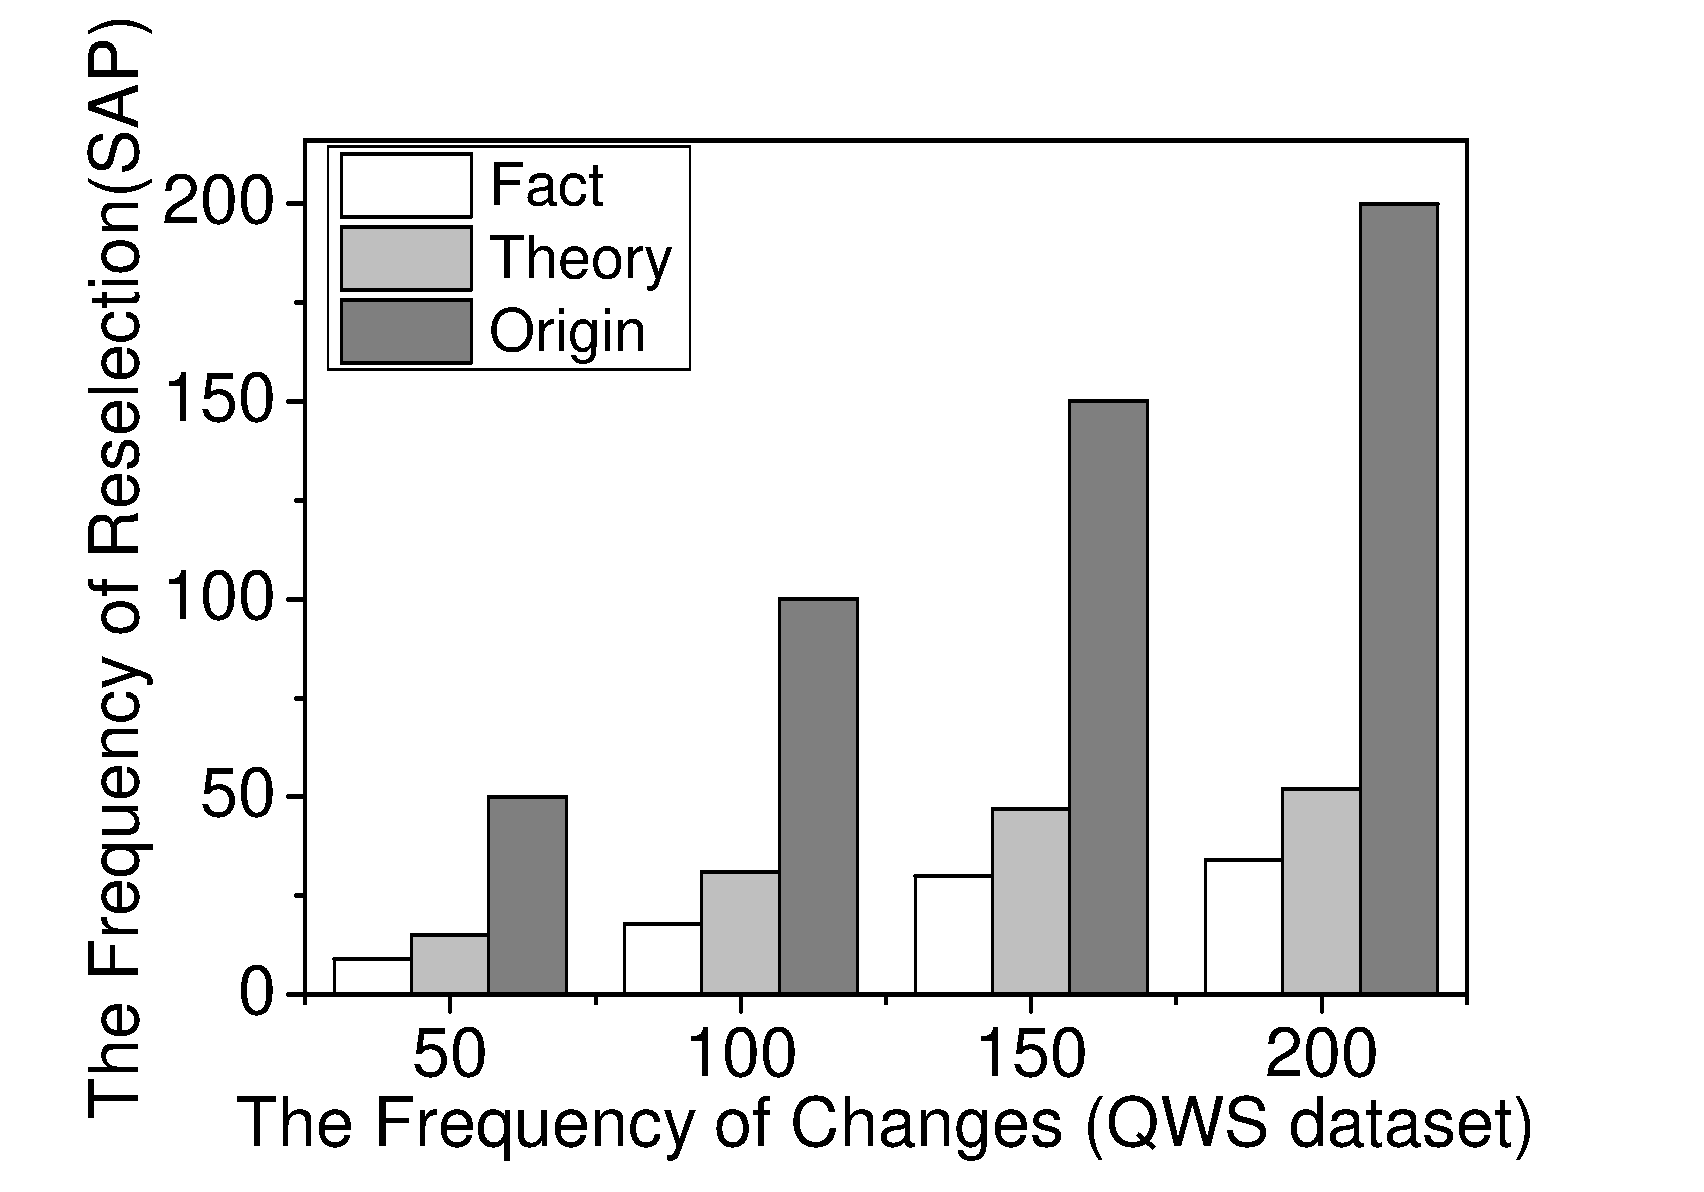
\includegraphics[width=0.47\textwidth]{./FIGs/Experiments/cvr_computing/effectiveness/SAP/Fig_Effect_QWS_SAP.pdf} \label{F:Fig_Exp_Effect_QWS_SAP} }
    \hspace{0.05in}
    \subfigure[] { 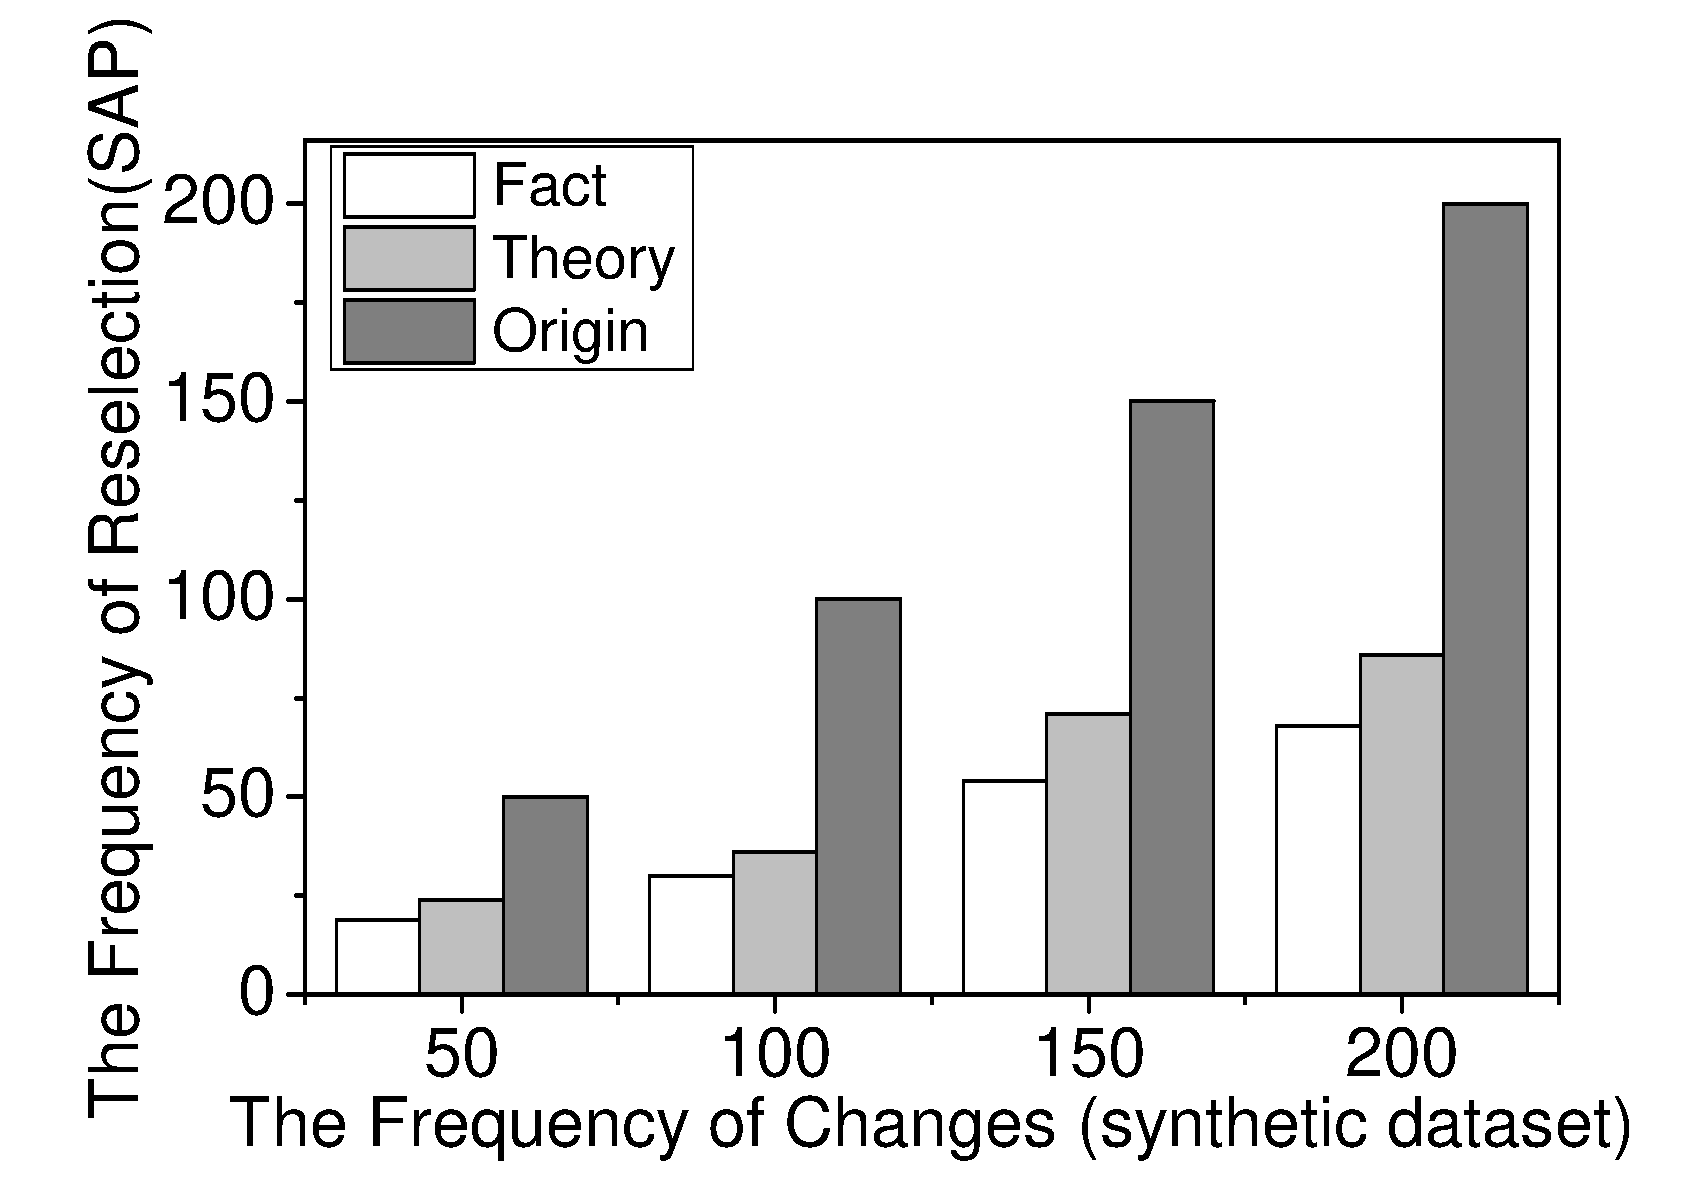
\includegraphics[width=0.47\textwidth,height=2.15in]{./FIGs/Experiments/cvr_computing/effectiveness/SAP/Fig_Effect_Random_SAP.pdf} \label{F:Fig_Exp_Effect_Random_SAP} }
    \caption{SVR~应用于重选~SAP}
    \label{F:Fig_Exp Effect_SAP}
  \end{minipage}%
\end{figure*}

\begin{figure*}[!thb]
 \begin{minipage}[b]{1\linewidth} % 如果一行放2个图,用0.5,如果3 个图,用0.33
    \centering
    \subfigure[] { 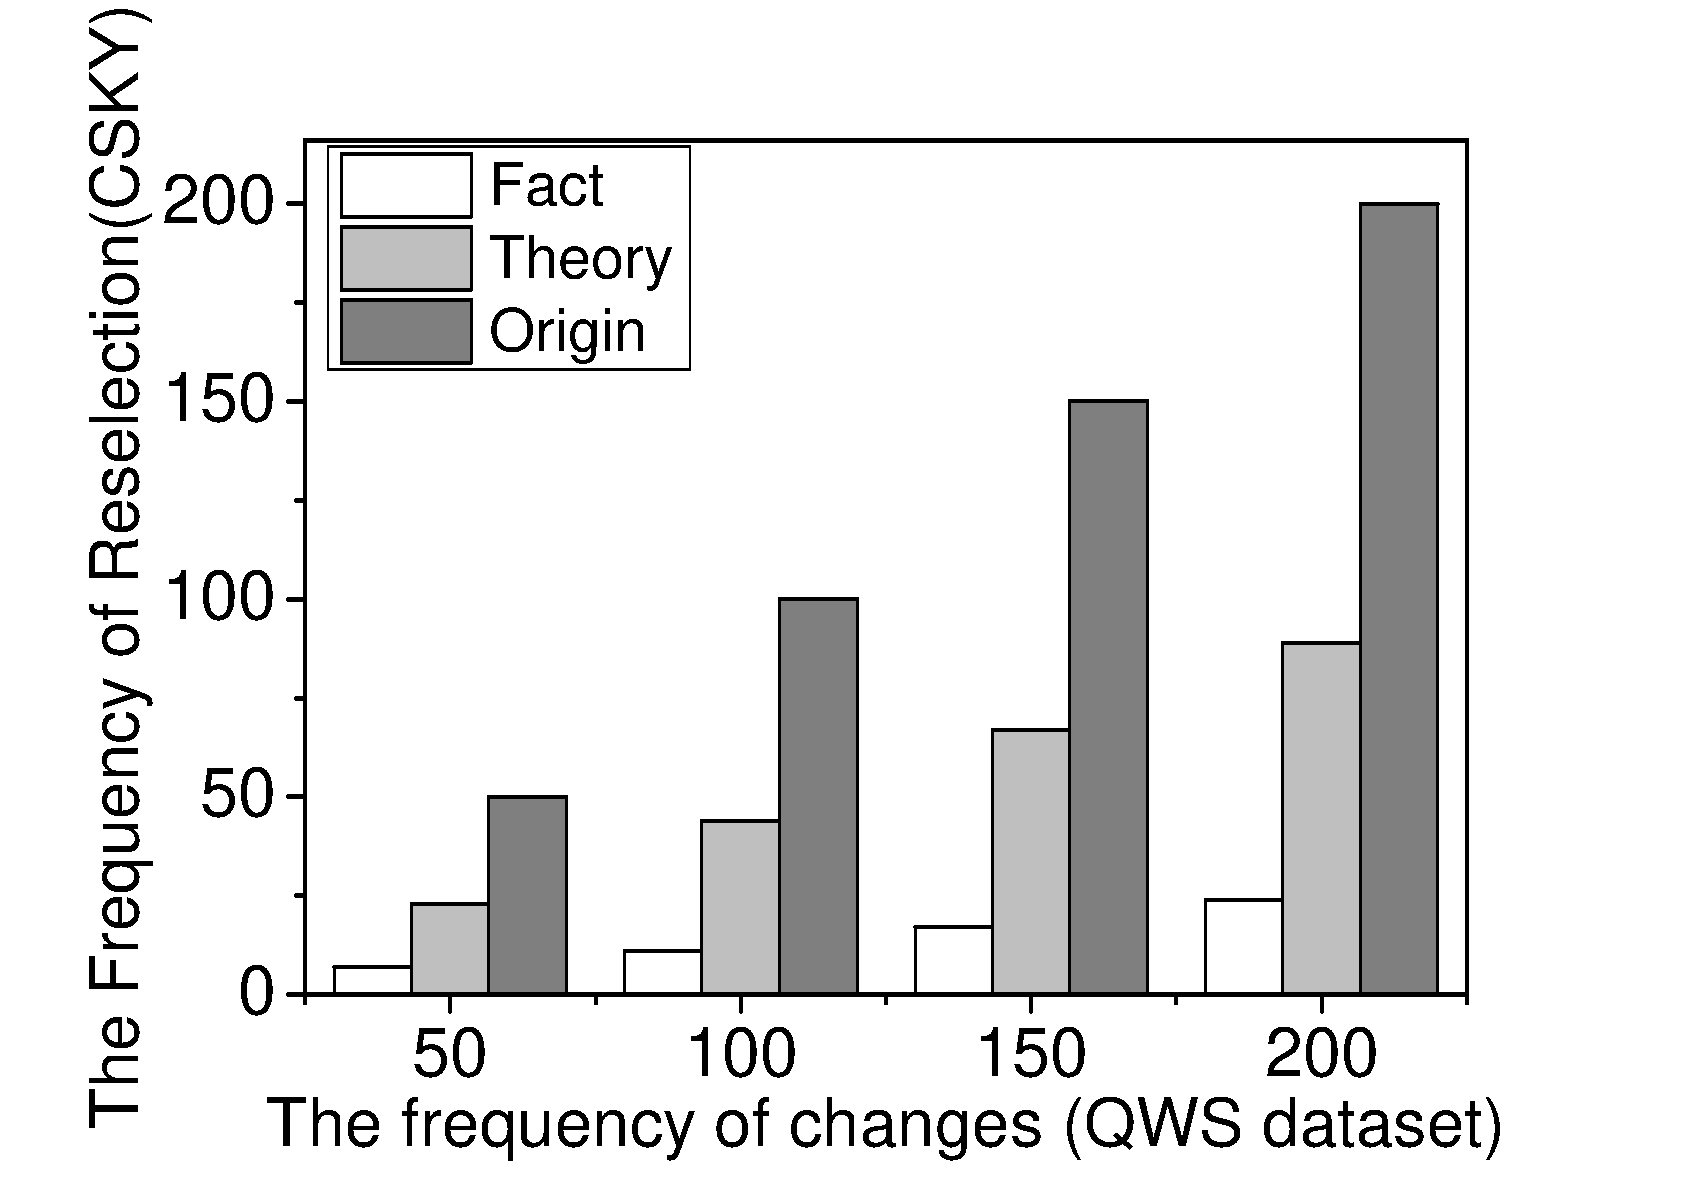
\includegraphics[width=0.47\textwidth]{./FIGs/Experiments/cvr_computing/effectiveness/CSKY/Fig_Effect_QWS_CSKY.pdf} \label{F:Fig_Exp_Effect_QWS_CSKY} }
    \hspace{0.05in}
    \subfigure[] { 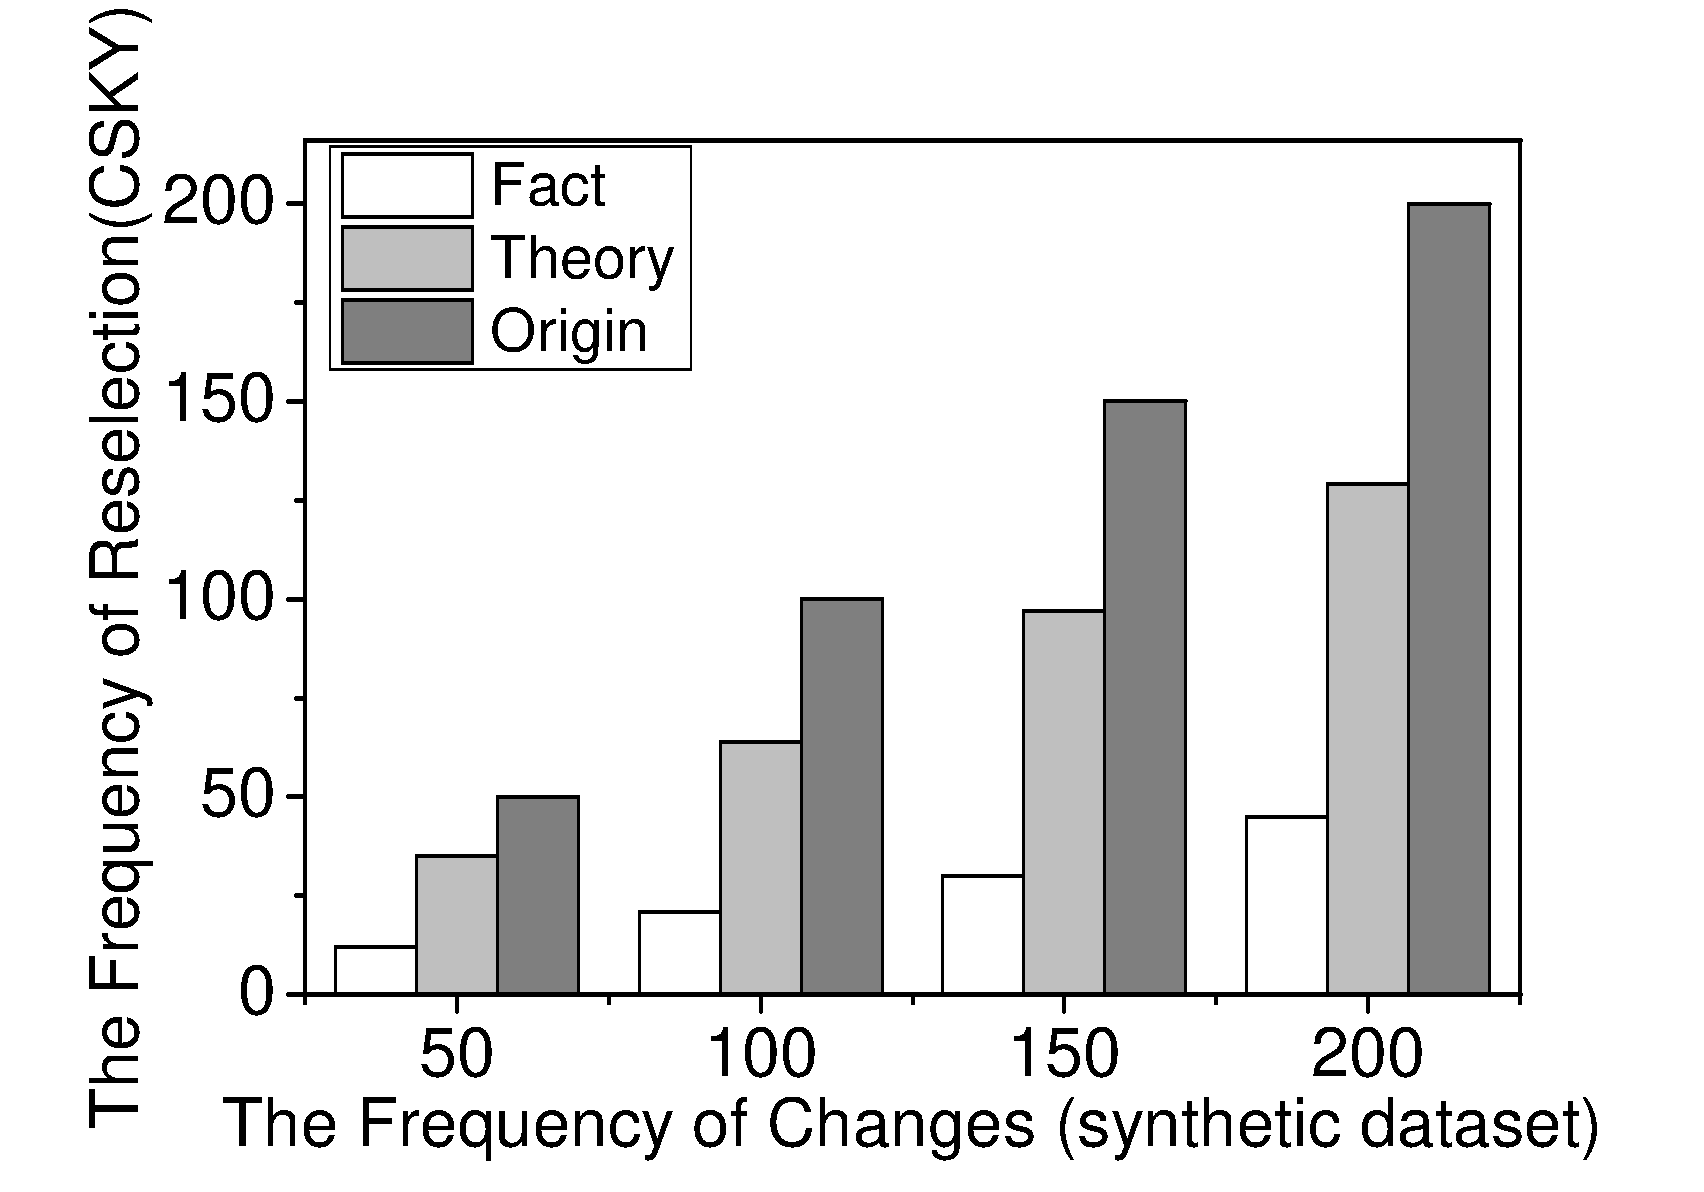
\includegraphics[width=0.47\textwidth,height=2.15in]{./FIGs/Experiments/cvr_computing/effectiveness/CSKY/Fig_Effect_Random_CSKY.pdf} \label{F:Fig_Exp_Effect_Random_CSKY} }
    \caption{SVR~应用于重选~CSKY}
    \label{F:Fig_Exp Effect_CSKY}
  \end{minipage}%
\end{figure*}


\subsubsection{实验二:误判率}

在本实验中,我们将通过多次改变~QoS~关联值,来统计用我们的方法需要重新运行选择的次数(Theory),并统计实际需要重新计算的次数(Fact),分析误判率(\underline{F}alse \underline{P}ositive \underline{R}ate,~FPR)。我们分别使用QWS~数据集以及系统生成的数据集,QoS~属性维度设置为~3,抽象服务的数量设置为~3,候选服务集合的大小设置~300,关联比重设置为~0.5,我们系统的改变关联值,分别改变~50,~100,~150,~200次。实验结果如图~\ref{F:Fig_Exp Effect_Rate_FP}~ 所示。

\begin{equation}
FPR = 1 - \frac{Fact}{Theory}
\label{E:EQ_FPR}
\end{equation}

\begin{figure*}[!thb]
 \begin{minipage}[b]{1\linewidth} % 如果一行放2个图,用0.5,如果3 个图,用0.33
    \centering
    \subfigure[SVR~应用于重选~SAP~的~FPR] { 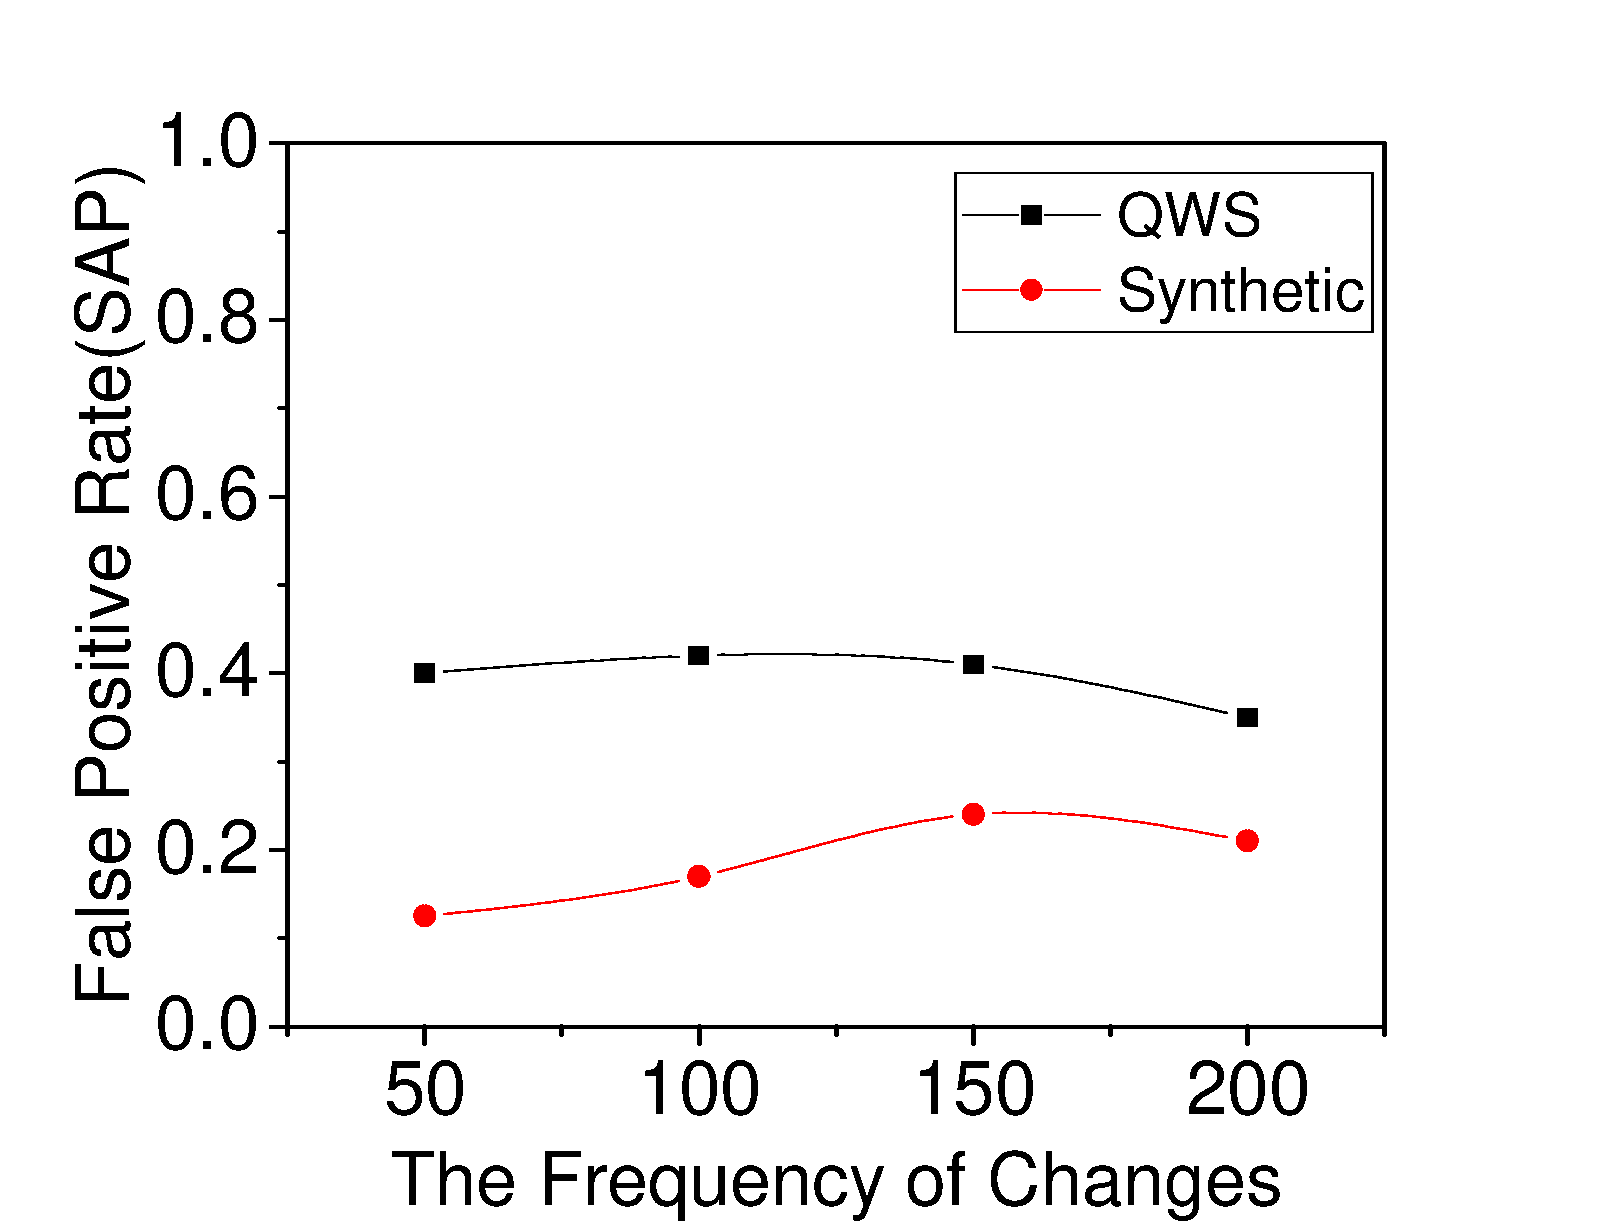
\includegraphics[width=0.47\textwidth]{./FIGs/Experiments/cvr_computing/effectiveness/SAP/Fig_Effect_SAP_Rate_FP.pdf} \label{F:Fig_Exp_Effect_SAP_Rate_FP} }
    \hspace{0.05in}
    \subfigure[SVR~应用于重选~CSKY~的~FPR] { 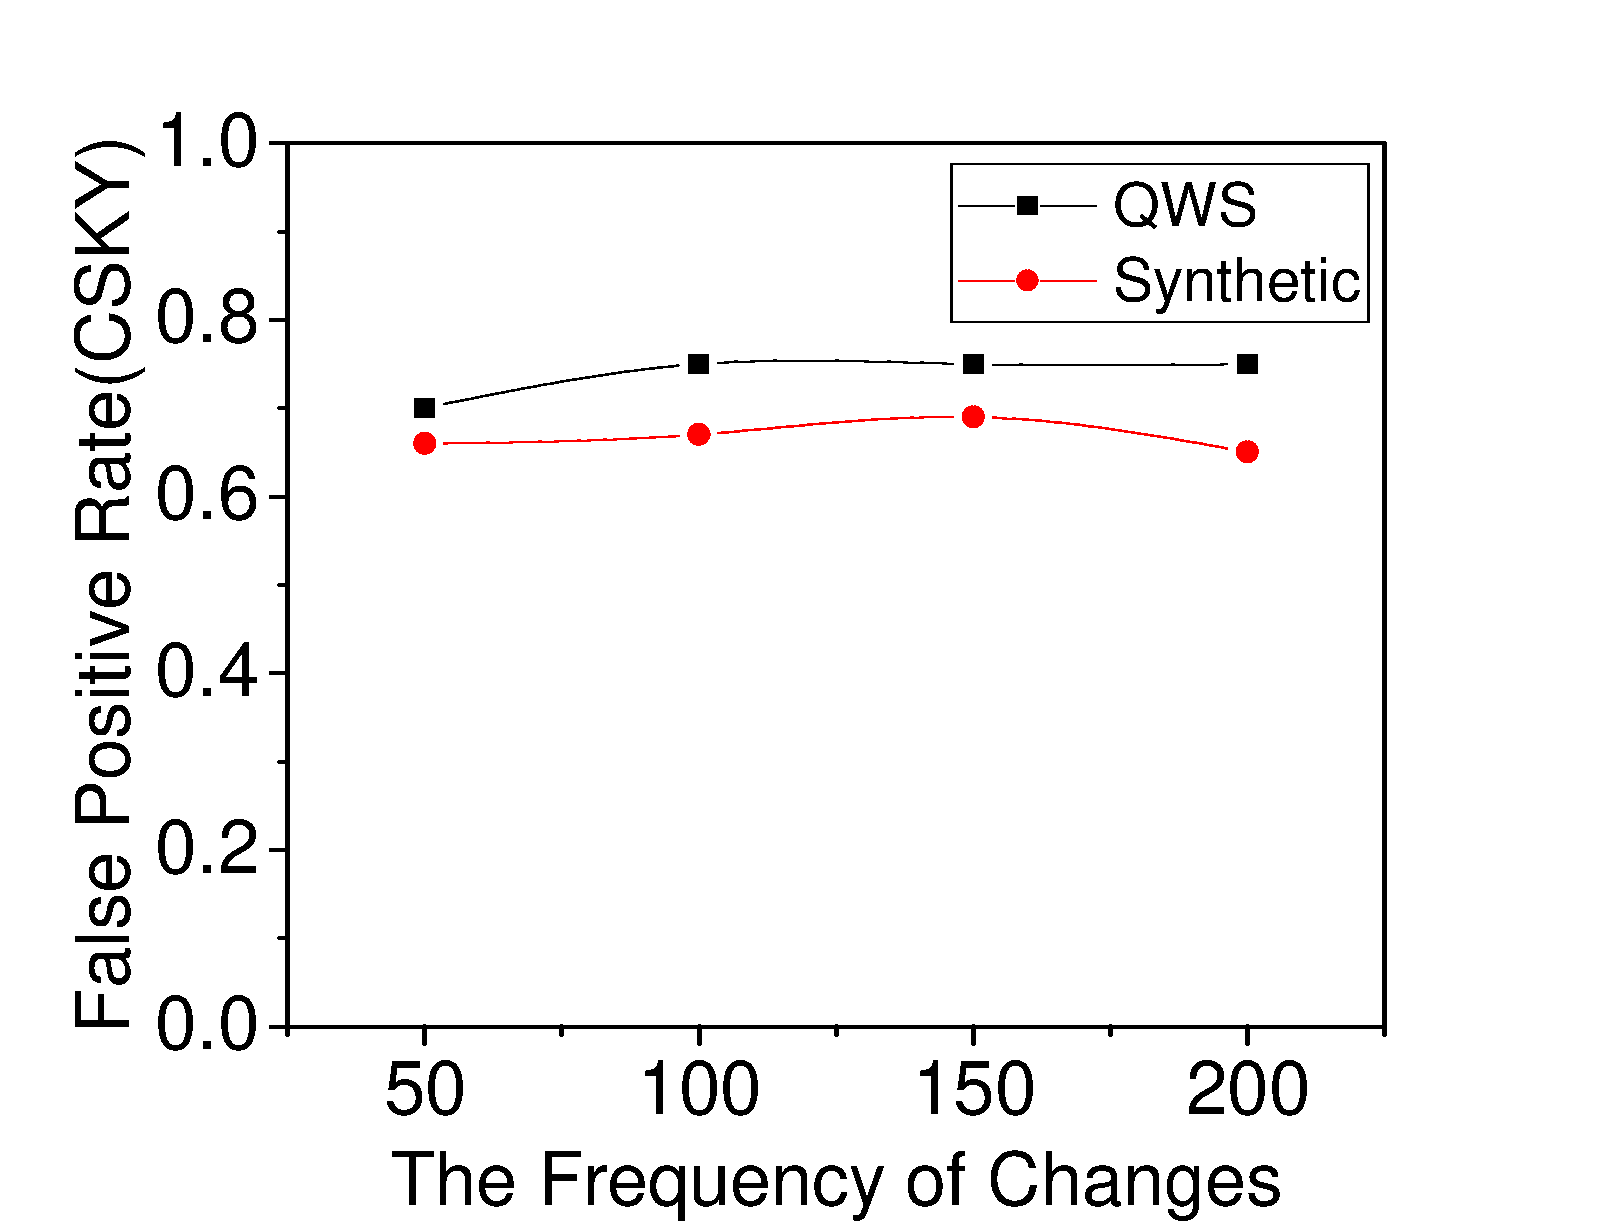
\includegraphics[width=0.47\textwidth]{./FIGs/Experiments/cvr_computing/effectiveness/CSKY/Fig_Effect_CSKY_Rate_FP.pdf} \label{F:Fig_Exp_Effect_CSKY_Rate_FP} }
    \caption{SVR~应用于重选的~FPR}
    \label{F:Fig_Exp Effect_Rate_FP}
  \end{minipage}%
\end{figure*}



\subsubsection{实验三:更新~SVR~的时间 \textbf{\emph{vs}} 重新选择~SAP~的时间}

通过本实验我们想验证,我们的更新~SVR~的时间要比重新选择~SAP~的时间快,来证明我们的更新是有意义的。我们分别使用QWS~数据集以及系统生成的数据集,QoS~属性维度设置为3,抽象服务的数量设置为~3,候选服务集合的大小设置~500,关联比重分别设置为~0.2 到~0.9,我们分别记录更新更新~SVR~ 的时间以及重新选择~SAP~的时间。实验结果如图~\ref{F:Fig_Exp Effect_UpdateBoundCompare}~ 所示。


\begin{figure*}[!thb]
 \begin{minipage}[b]{1\linewidth} % 如果一行放2个图,用0.5,如果3 个图,用0.33
    \centering
    \subfigure[] { 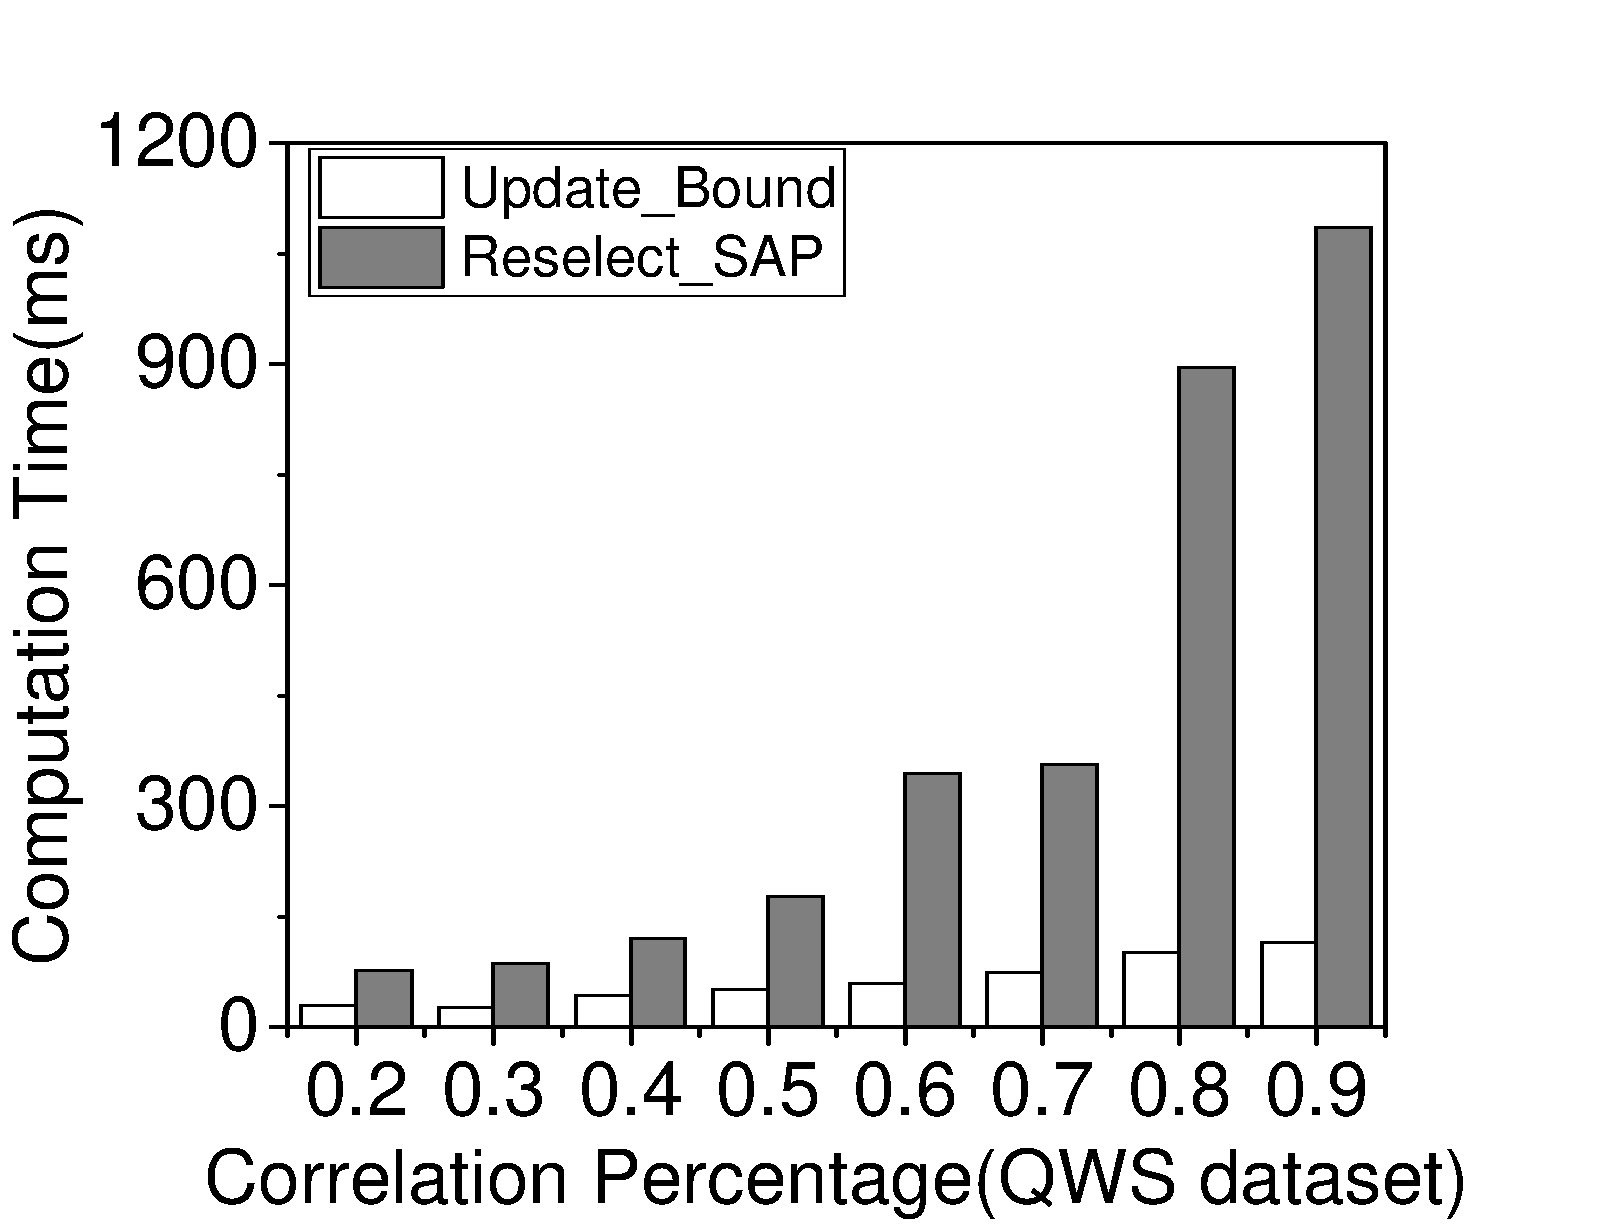
\includegraphics[width=0.47\textwidth]{./FIGs/Experiments/cvr_computing/effectiveness/Effect_UpdateBoundCompare500_QWS.pdf} \label{F:Fig_Exp_Effect_UpdateBoundCompare_QWS} }
    \hspace{0.05in}
    \subfigure[] { 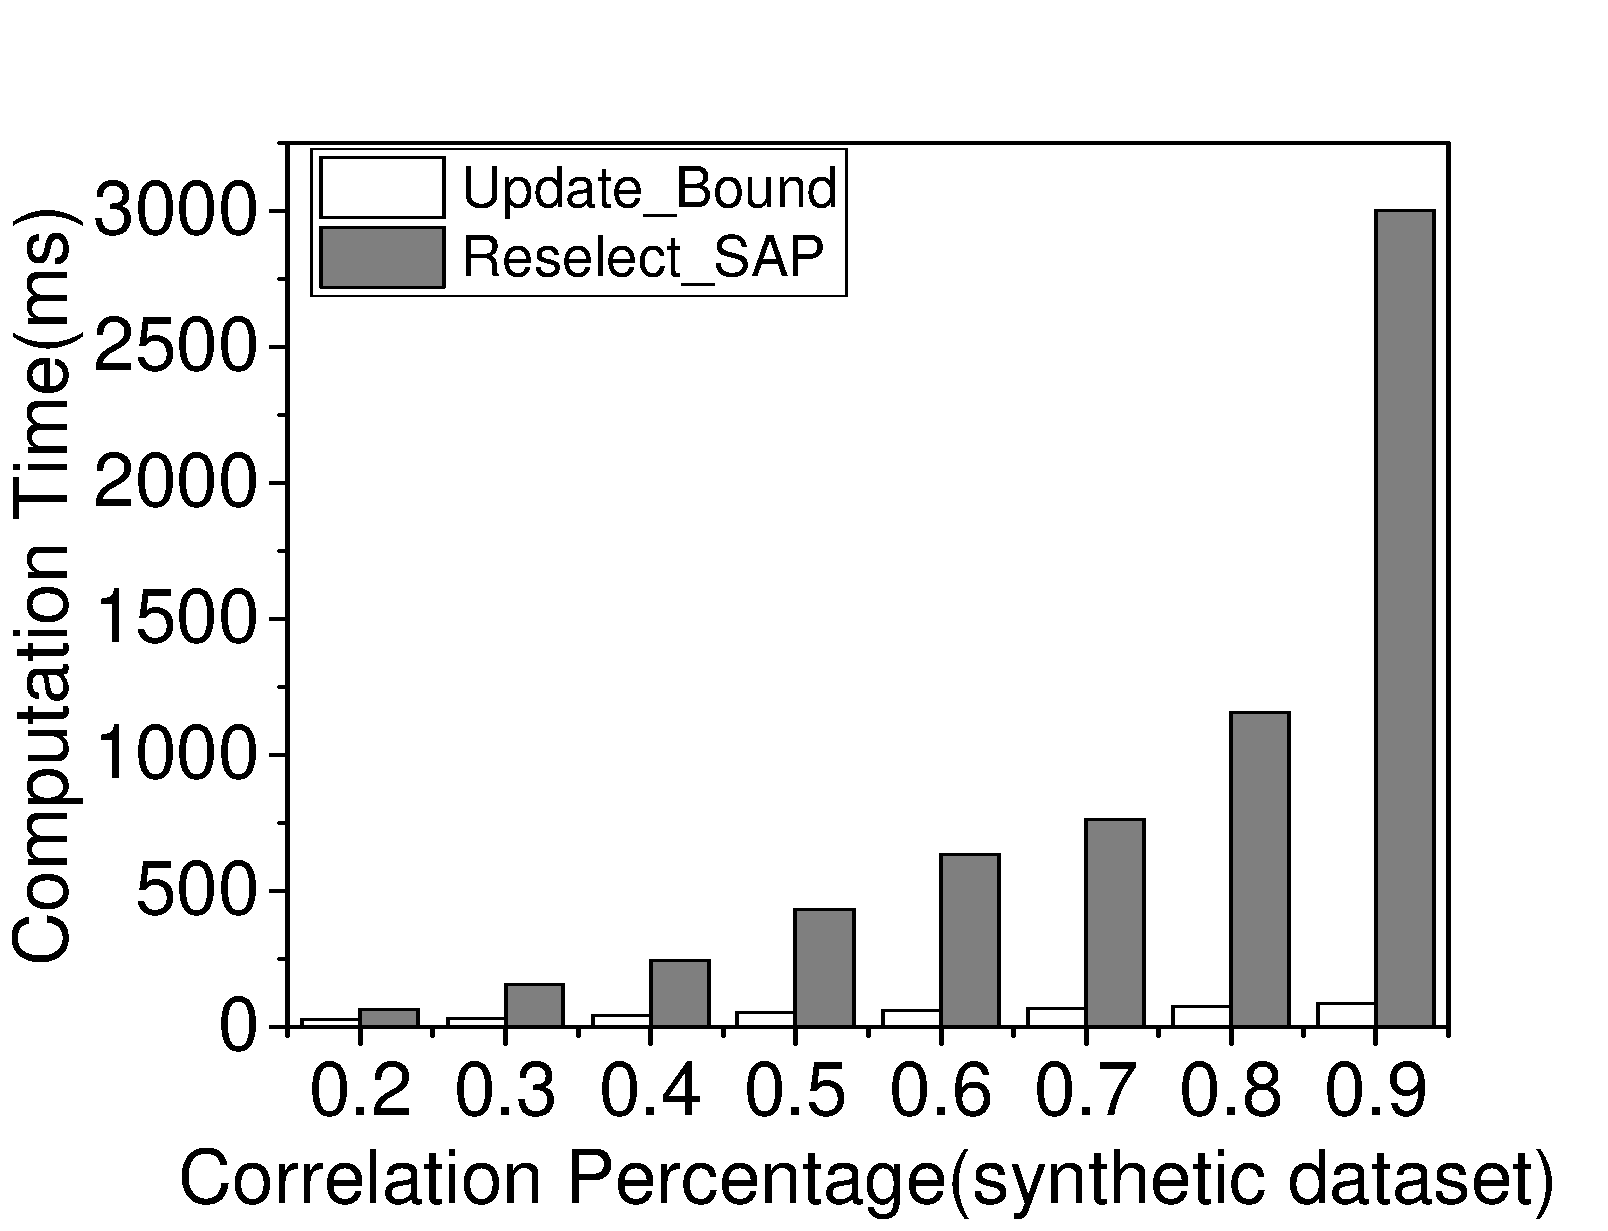
\includegraphics[width=0.47\textwidth,height=2.28in]{./FIGs/Experiments/cvr_computing/effectiveness/Effect_UpdateBoundCompare500_Synthetic.pdf} \label{F:Fig_Exp_Effect_UpdateBoundCompare_SYN} }
    \caption{更新~SVR~的时间 \textbf{\emph{vs}} 重新选择~SAP~的时间}
    \label{F:Fig_Exp Effect_UpdateBoundCompare}
  \end{minipage}%
\end{figure*}

\subsection{效率实验}
\subsubsection{实验四:计算~SVR~时间}

通过本实验我们想展示我们方法计算~SVR~所需的时间。我们分别使用QWS~ 数据集以及系统生成的数据集,QoS~属性维度设置为~3,抽象服务的数量设置为~3,候选服务集合的大小分别设置为~200,~300,~500,关联比重分别设置为~0.2 到~0.9。实验结果如图~\ref{F:Fig_Exp Efficient_Bound}~所示。

\begin{figure*}[!thb]
 \begin{minipage}[b]{1\linewidth} % 如果一行放2个图,用0.5,如果3 个图,用0.33
    \centering
    \subfigure[] { 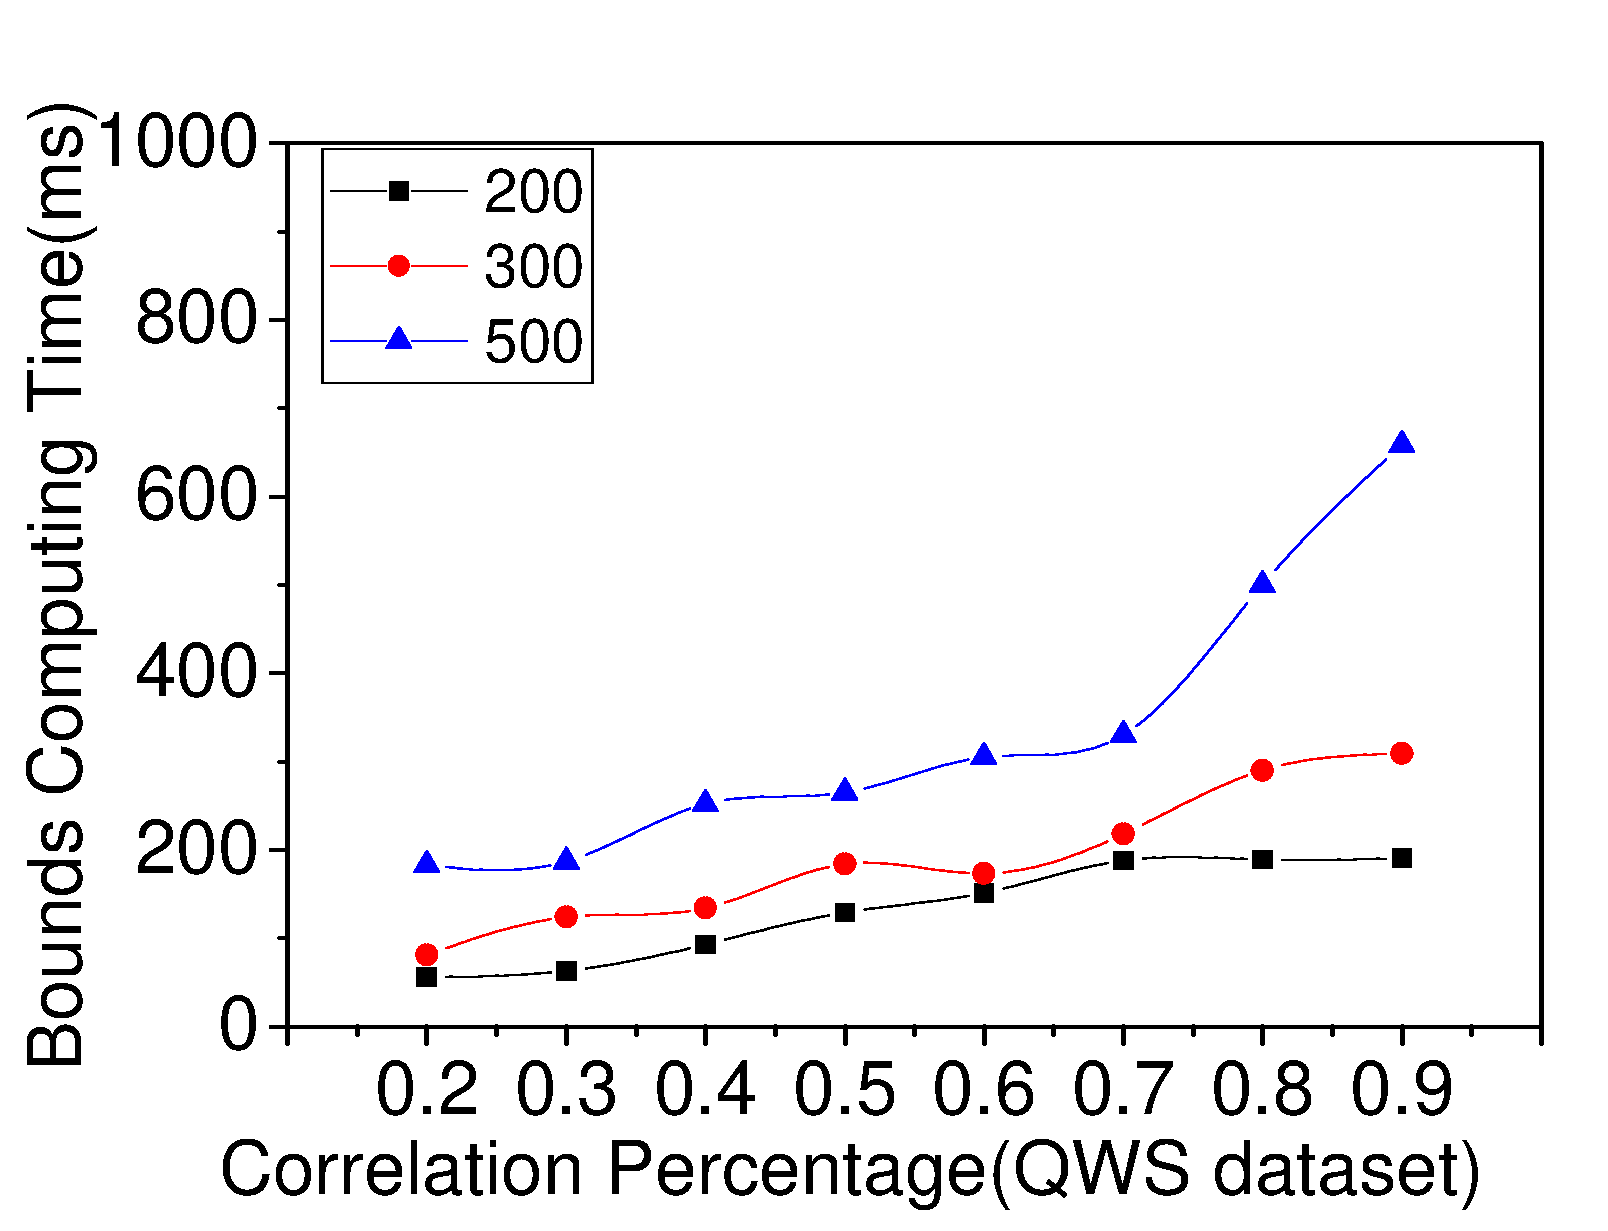
\includegraphics[width=0.47\textwidth]{./FIGs/Experiments/cvr_computing/efficiency/Fig_Efficient_Bound_QWS.pdf} \label{F:Fig_Exp_Efficient_Bound_QWS} }
    \hspace{0.05in}
    \subfigure[] { 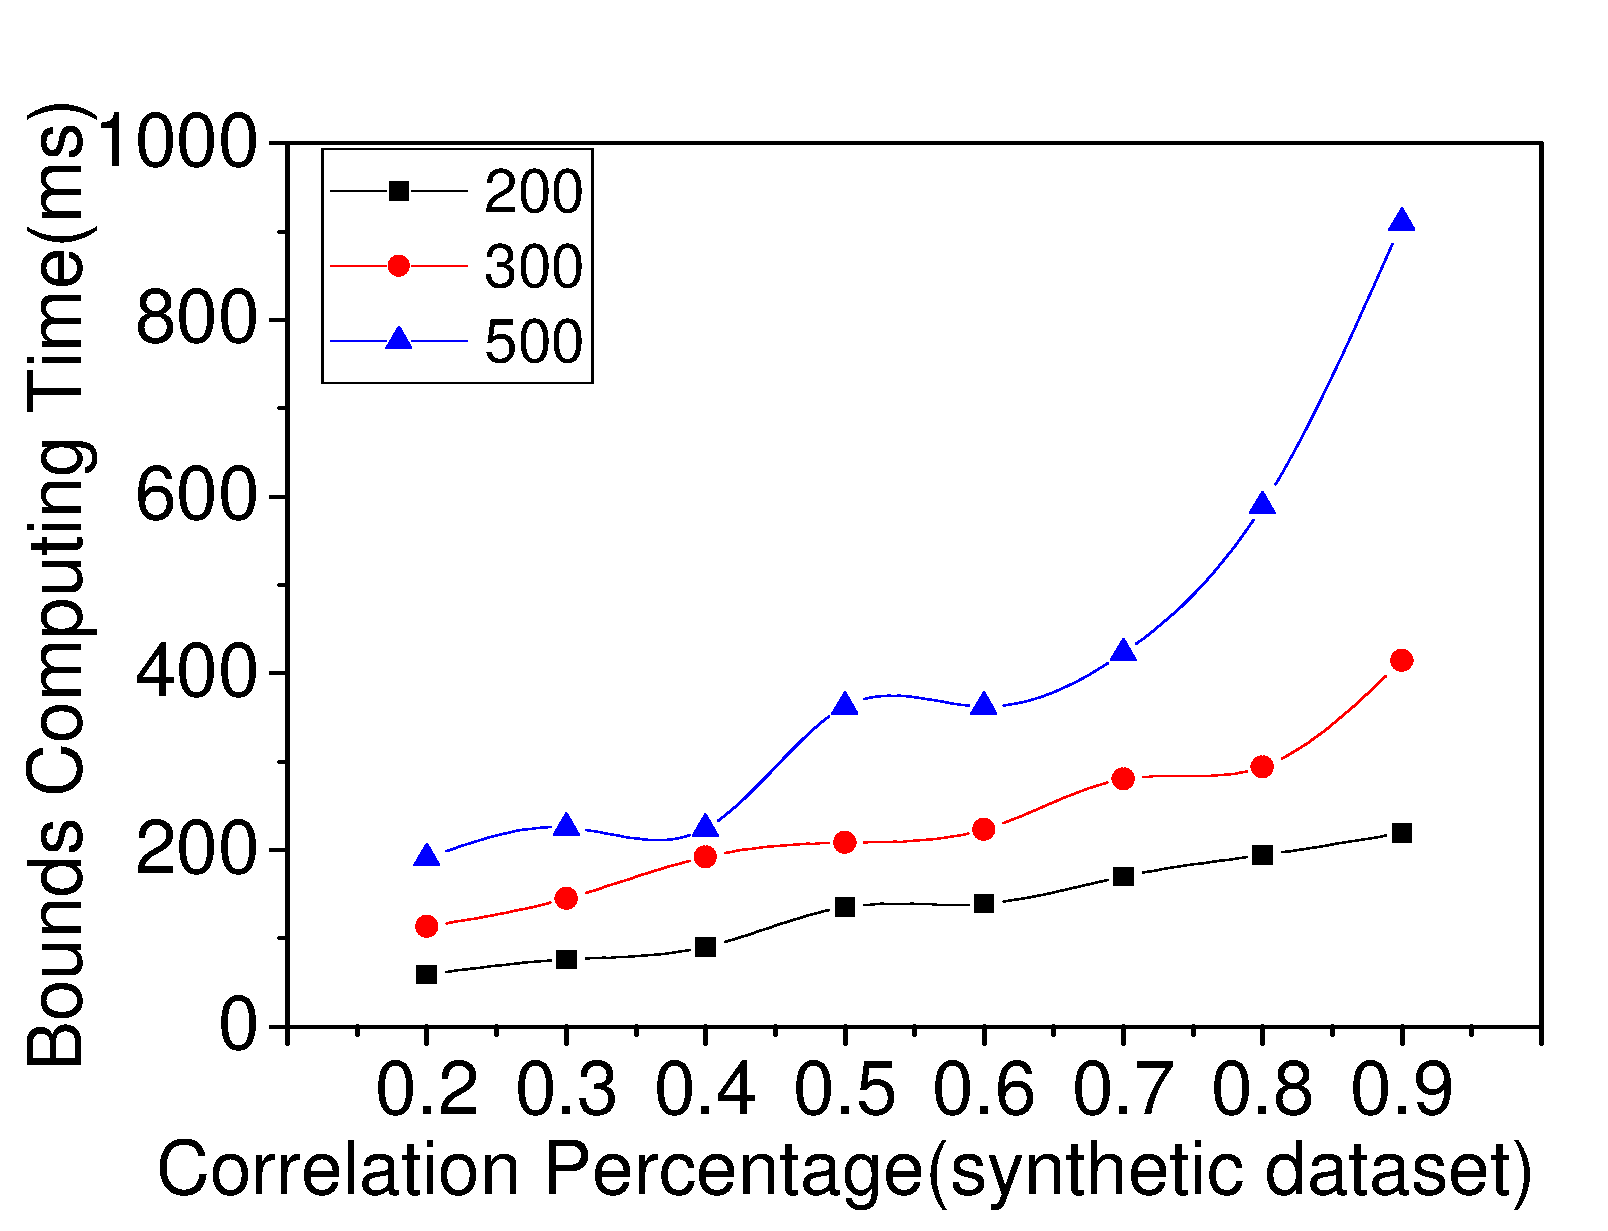
\includegraphics[width=0.47\textwidth]{./FIGs/Experiments/cvr_computing/efficiency/Fig_Efficient_Bound_Synthetic.pdf} \label{F:Fig_Exp_Efficient_Bound_Synthetic} }
    \caption{计算~SVR~时间}
    \label{F:Fig_Exp Efficient_Bound}
  \end{minipage}%
\end{figure*}

\subsubsection{实验五:更新~SVR~时间}

通过本实验我们想展示我们方法更新~SVR~所需的时间。我们分别使用QWS~ 数据集以及系统生成的数据集,QoS~属性维度设置为~3,抽象服务的数量设置为~3,候选服务集合的大小分别设置为~200,~300,~500,关联比重分别设置为~0.2 到~0.9。实验结果如图~\ref{F:Fig_Exp Efficient_UpdateBound}~ 所示。

\begin{figure*}[!thb]
 \begin{minipage}[b]{1\linewidth} % 如果一行放2个图,用0.5,如果3 个图,用0.33
    \centering
    \subfigure[] { 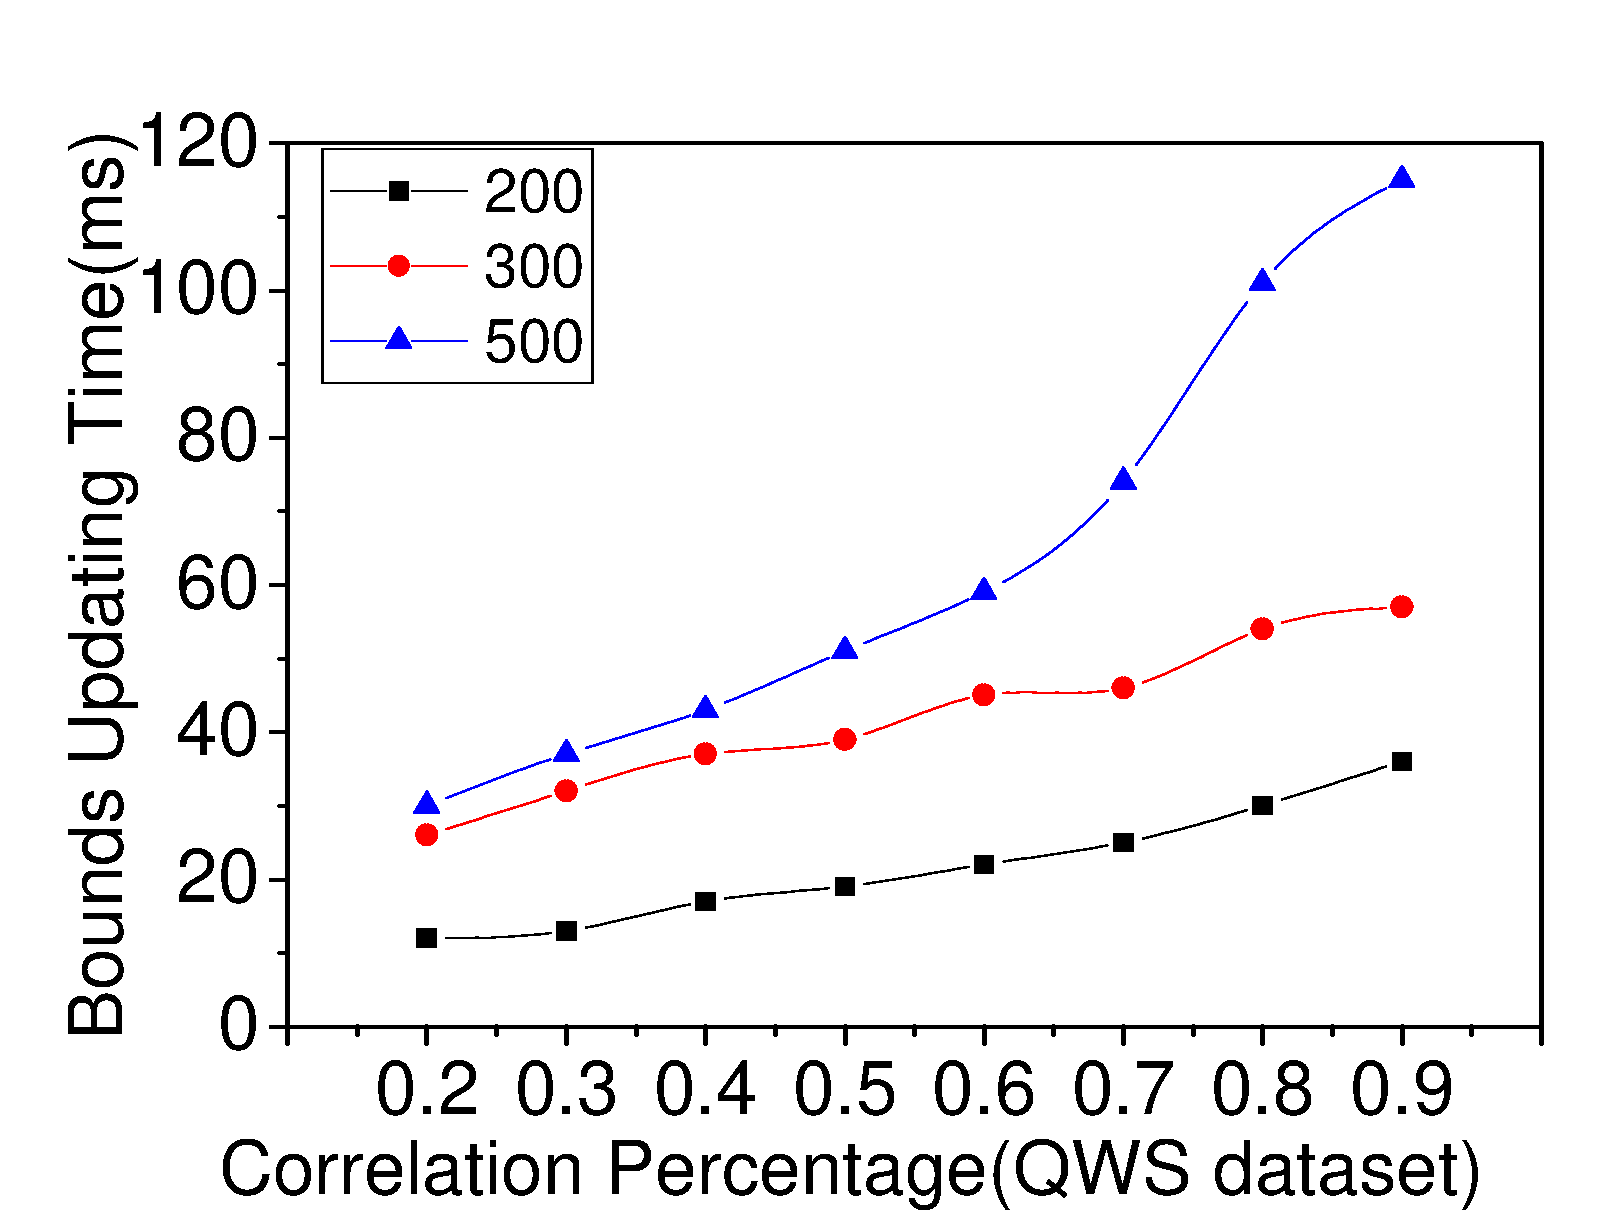
\includegraphics[width=0.47\textwidth]{./FIGs/Experiments/cvr_computing/efficiency/Fig_Efficient_UpdateBound_QWS.pdf} \label{F:Fig_Exp_Efficient_UpdateBound_QWS} }
    \hspace{0.05in}
    \subfigure[] { 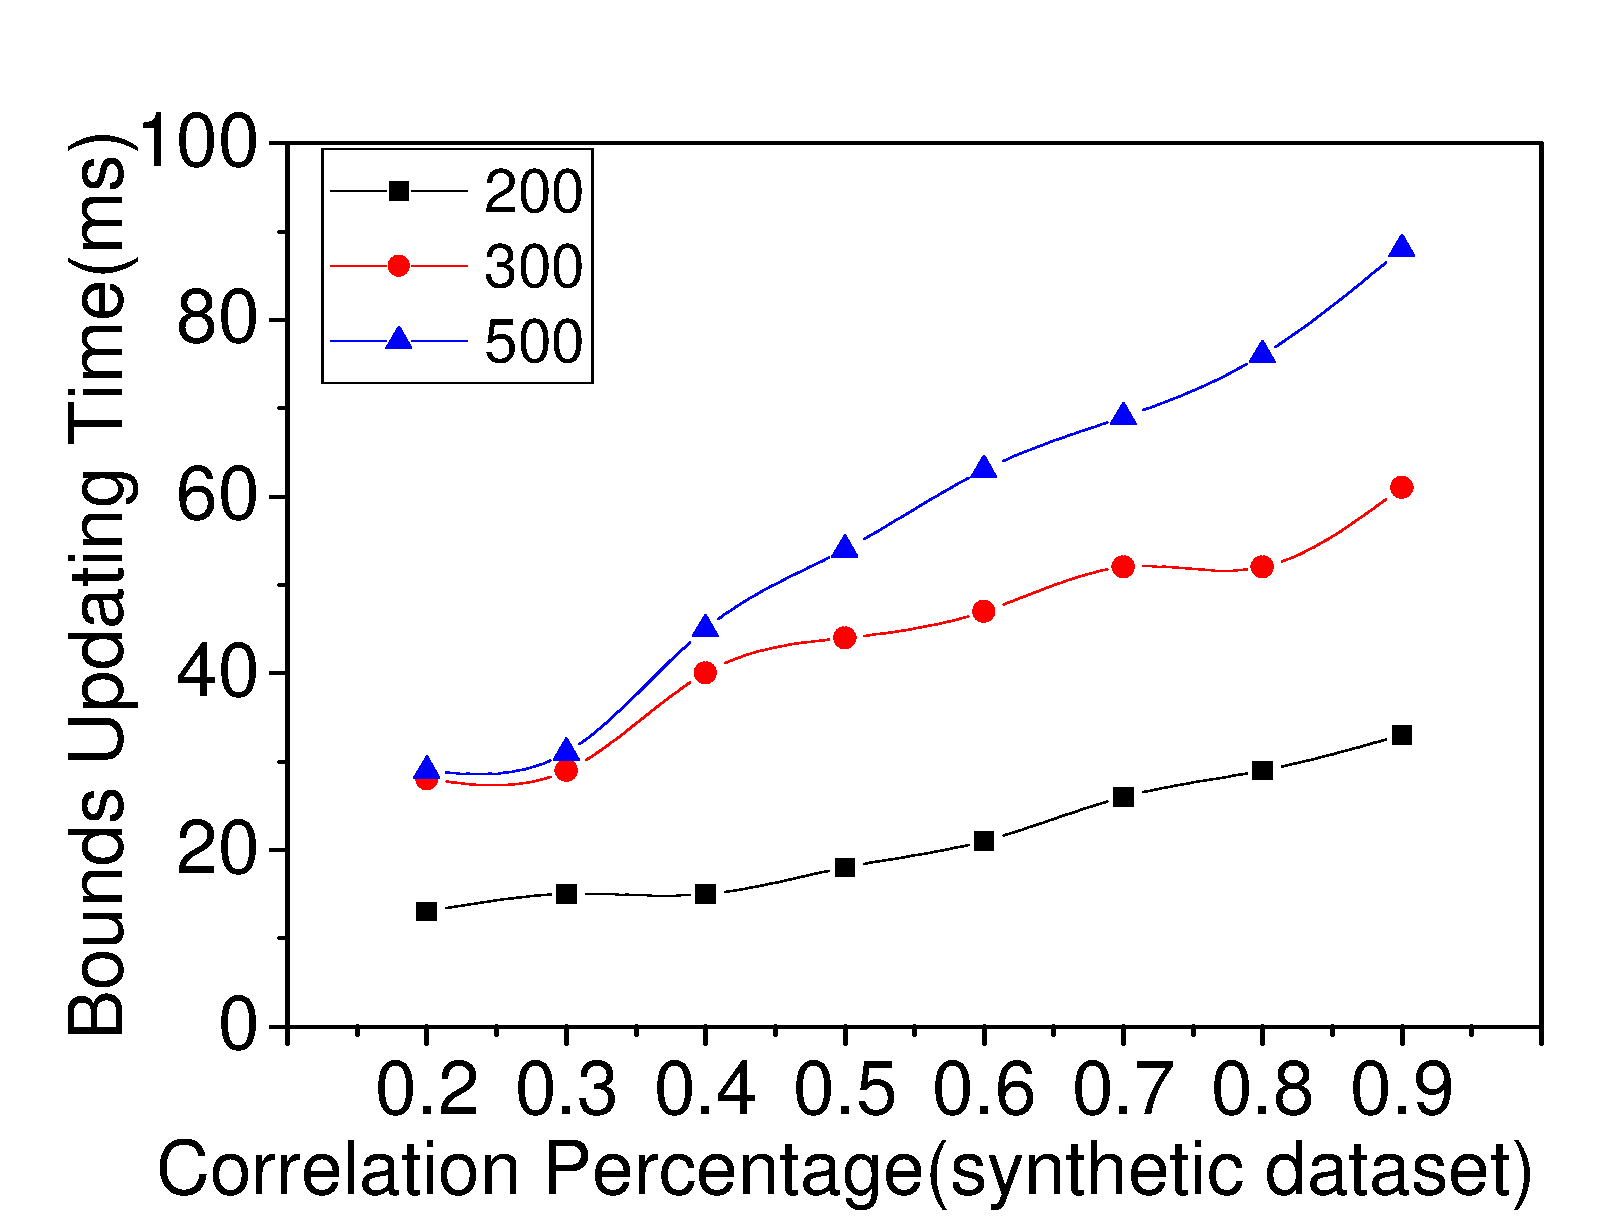
\includegraphics[width=0.47\textwidth]{./FIGs/Experiments/cvr_computing/efficiency/Fig_Efficient_UpdateBound_Synthetic.pdf} \label{F:Fig_Exp_Efficient_UpdateBound_Synthetic} }
    \caption{更新~SVR~时间}
    \label{F:Fig_Exp Efficient_UpdateBound}
  \end{minipage}%
\end{figure*}

\section{本章小结}

我们在本章定义了移动环境导致~Web~服务关联值不确定时如何计算组合服务~Skyline的问题,我们提出了安全值范围的概念,并利用安全值范围在一定程度上降低了~SAP~以及~CSKY~重新计算的次数,提高了组合服务代理的运行效率。最后,我们通过一些列实验来分析我们方法的有效性以及效率。